% Options for packages loaded elsewhere
\PassOptionsToPackage{unicode}{hyperref}
\PassOptionsToPackage{hyphens}{url}
\PassOptionsToPackage{dvipsnames,svgnames,x11names}{xcolor}
%
\documentclass[
  letterpaper,
  DIV=11,
  numbers=noendperiod]{scrartcl}

\usepackage{amsmath,amssymb}
\usepackage{iftex}
\ifPDFTeX
  \usepackage[T1]{fontenc}
  \usepackage[utf8]{inputenc}
  \usepackage{textcomp} % provide euro and other symbols
\else % if luatex or xetex
  \usepackage{unicode-math}
  \defaultfontfeatures{Scale=MatchLowercase}
  \defaultfontfeatures[\rmfamily]{Ligatures=TeX,Scale=1}
\fi
\usepackage{lmodern}
\ifPDFTeX\else  
    % xetex/luatex font selection
\fi
% Use upquote if available, for straight quotes in verbatim environments
\IfFileExists{upquote.sty}{\usepackage{upquote}}{}
\IfFileExists{microtype.sty}{% use microtype if available
  \usepackage[]{microtype}
  \UseMicrotypeSet[protrusion]{basicmath} % disable protrusion for tt fonts
}{}
\makeatletter
\@ifundefined{KOMAClassName}{% if non-KOMA class
  \IfFileExists{parskip.sty}{%
    \usepackage{parskip}
  }{% else
    \setlength{\parindent}{0pt}
    \setlength{\parskip}{6pt plus 2pt minus 1pt}}
}{% if KOMA class
  \KOMAoptions{parskip=half}}
\makeatother
\usepackage{xcolor}
\setlength{\emergencystretch}{3em} % prevent overfull lines
\setcounter{secnumdepth}{-\maxdimen} % remove section numbering
% Make \paragraph and \subparagraph free-standing
\ifx\paragraph\undefined\else
  \let\oldparagraph\paragraph
  \renewcommand{\paragraph}[1]{\oldparagraph{#1}\mbox{}}
\fi
\ifx\subparagraph\undefined\else
  \let\oldsubparagraph\subparagraph
  \renewcommand{\subparagraph}[1]{\oldsubparagraph{#1}\mbox{}}
\fi

\usepackage{color}
\usepackage{fancyvrb}
\newcommand{\VerbBar}{|}
\newcommand{\VERB}{\Verb[commandchars=\\\{\}]}
\DefineVerbatimEnvironment{Highlighting}{Verbatim}{commandchars=\\\{\}}
% Add ',fontsize=\small' for more characters per line
\usepackage{framed}
\definecolor{shadecolor}{RGB}{241,243,245}
\newenvironment{Shaded}{\begin{snugshade}}{\end{snugshade}}
\newcommand{\AlertTok}[1]{\textcolor[rgb]{0.68,0.00,0.00}{#1}}
\newcommand{\AnnotationTok}[1]{\textcolor[rgb]{0.37,0.37,0.37}{#1}}
\newcommand{\AttributeTok}[1]{\textcolor[rgb]{0.40,0.45,0.13}{#1}}
\newcommand{\BaseNTok}[1]{\textcolor[rgb]{0.68,0.00,0.00}{#1}}
\newcommand{\BuiltInTok}[1]{\textcolor[rgb]{0.00,0.23,0.31}{#1}}
\newcommand{\CharTok}[1]{\textcolor[rgb]{0.13,0.47,0.30}{#1}}
\newcommand{\CommentTok}[1]{\textcolor[rgb]{0.37,0.37,0.37}{#1}}
\newcommand{\CommentVarTok}[1]{\textcolor[rgb]{0.37,0.37,0.37}{\textit{#1}}}
\newcommand{\ConstantTok}[1]{\textcolor[rgb]{0.56,0.35,0.01}{#1}}
\newcommand{\ControlFlowTok}[1]{\textcolor[rgb]{0.00,0.23,0.31}{#1}}
\newcommand{\DataTypeTok}[1]{\textcolor[rgb]{0.68,0.00,0.00}{#1}}
\newcommand{\DecValTok}[1]{\textcolor[rgb]{0.68,0.00,0.00}{#1}}
\newcommand{\DocumentationTok}[1]{\textcolor[rgb]{0.37,0.37,0.37}{\textit{#1}}}
\newcommand{\ErrorTok}[1]{\textcolor[rgb]{0.68,0.00,0.00}{#1}}
\newcommand{\ExtensionTok}[1]{\textcolor[rgb]{0.00,0.23,0.31}{#1}}
\newcommand{\FloatTok}[1]{\textcolor[rgb]{0.68,0.00,0.00}{#1}}
\newcommand{\FunctionTok}[1]{\textcolor[rgb]{0.28,0.35,0.67}{#1}}
\newcommand{\ImportTok}[1]{\textcolor[rgb]{0.00,0.46,0.62}{#1}}
\newcommand{\InformationTok}[1]{\textcolor[rgb]{0.37,0.37,0.37}{#1}}
\newcommand{\KeywordTok}[1]{\textcolor[rgb]{0.00,0.23,0.31}{#1}}
\newcommand{\NormalTok}[1]{\textcolor[rgb]{0.00,0.23,0.31}{#1}}
\newcommand{\OperatorTok}[1]{\textcolor[rgb]{0.37,0.37,0.37}{#1}}
\newcommand{\OtherTok}[1]{\textcolor[rgb]{0.00,0.23,0.31}{#1}}
\newcommand{\PreprocessorTok}[1]{\textcolor[rgb]{0.68,0.00,0.00}{#1}}
\newcommand{\RegionMarkerTok}[1]{\textcolor[rgb]{0.00,0.23,0.31}{#1}}
\newcommand{\SpecialCharTok}[1]{\textcolor[rgb]{0.37,0.37,0.37}{#1}}
\newcommand{\SpecialStringTok}[1]{\textcolor[rgb]{0.13,0.47,0.30}{#1}}
\newcommand{\StringTok}[1]{\textcolor[rgb]{0.13,0.47,0.30}{#1}}
\newcommand{\VariableTok}[1]{\textcolor[rgb]{0.07,0.07,0.07}{#1}}
\newcommand{\VerbatimStringTok}[1]{\textcolor[rgb]{0.13,0.47,0.30}{#1}}
\newcommand{\WarningTok}[1]{\textcolor[rgb]{0.37,0.37,0.37}{\textit{#1}}}

\providecommand{\tightlist}{%
  \setlength{\itemsep}{0pt}\setlength{\parskip}{0pt}}\usepackage{longtable,booktabs,array}
\usepackage{calc} % for calculating minipage widths
% Correct order of tables after \paragraph or \subparagraph
\usepackage{etoolbox}
\makeatletter
\patchcmd\longtable{\par}{\if@noskipsec\mbox{}\fi\par}{}{}
\makeatother
% Allow footnotes in longtable head/foot
\IfFileExists{footnotehyper.sty}{\usepackage{footnotehyper}}{\usepackage{footnote}}
\makesavenoteenv{longtable}
\usepackage{graphicx}
\makeatletter
\def\maxwidth{\ifdim\Gin@nat@width>\linewidth\linewidth\else\Gin@nat@width\fi}
\def\maxheight{\ifdim\Gin@nat@height>\textheight\textheight\else\Gin@nat@height\fi}
\makeatother
% Scale images if necessary, so that they will not overflow the page
% margins by default, and it is still possible to overwrite the defaults
% using explicit options in \includegraphics[width, height, ...]{}
\setkeys{Gin}{width=\maxwidth,height=\maxheight,keepaspectratio}
% Set default figure placement to htbp
\makeatletter
\def\fps@figure{htbp}
\makeatother
\newlength{\cslhangindent}
\setlength{\cslhangindent}{1.5em}
\newlength{\csllabelwidth}
\setlength{\csllabelwidth}{3em}
\newlength{\cslentryspacingunit} % times entry-spacing
\setlength{\cslentryspacingunit}{\parskip}
\newenvironment{CSLReferences}[2] % #1 hanging-ident, #2 entry spacing
 {% don't indent paragraphs
  \setlength{\parindent}{0pt}
  % turn on hanging indent if param 1 is 1
  \ifodd #1
  \let\oldpar\par
  \def\par{\hangindent=\cslhangindent\oldpar}
  \fi
  % set entry spacing
  \setlength{\parskip}{#2\cslentryspacingunit}
 }%
 {}
\usepackage{calc}
\newcommand{\CSLBlock}[1]{#1\hfill\break}
\newcommand{\CSLLeftMargin}[1]{\parbox[t]{\csllabelwidth}{#1}}
\newcommand{\CSLRightInline}[1]{\parbox[t]{\linewidth - \csllabelwidth}{#1}\break}
\newcommand{\CSLIndent}[1]{\hspace{\cslhangindent}#1}

\usepackage{booktabs}
\usepackage{longtable}
\usepackage{array}
\usepackage{multirow}
\usepackage{wrapfig}
\usepackage{float}
\usepackage{colortbl}
\usepackage{pdflscape}
\usepackage{tabu}
\usepackage{threeparttable}
\usepackage{threeparttablex}
\usepackage[normalem]{ulem}
\usepackage{makecell}
\usepackage{xcolor}
\KOMAoption{captions}{tableheading}
\makeatletter
\makeatother
\makeatletter
\makeatother
\makeatletter
\@ifpackageloaded{caption}{}{\usepackage{caption}}
\AtBeginDocument{%
\ifdefined\contentsname
  \renewcommand*\contentsname{Table of contents}
\else
  \newcommand\contentsname{Table of contents}
\fi
\ifdefined\listfigurename
  \renewcommand*\listfigurename{List of Figures}
\else
  \newcommand\listfigurename{List of Figures}
\fi
\ifdefined\listtablename
  \renewcommand*\listtablename{List of Tables}
\else
  \newcommand\listtablename{List of Tables}
\fi
\ifdefined\figurename
  \renewcommand*\figurename{Figure}
\else
  \newcommand\figurename{Figure}
\fi
\ifdefined\tablename
  \renewcommand*\tablename{Table}
\else
  \newcommand\tablename{Table}
\fi
}
\@ifpackageloaded{float}{}{\usepackage{float}}
\floatstyle{ruled}
\@ifundefined{c@chapter}{\newfloat{codelisting}{h}{lop}}{\newfloat{codelisting}{h}{lop}[chapter]}
\floatname{codelisting}{Listing}
\newcommand*\listoflistings{\listof{codelisting}{List of Listings}}
\makeatother
\makeatletter
\@ifpackageloaded{caption}{}{\usepackage{caption}}
\@ifpackageloaded{subcaption}{}{\usepackage{subcaption}}
\makeatother
\makeatletter
\@ifpackageloaded{tcolorbox}{}{\usepackage[skins,breakable]{tcolorbox}}
\makeatother
\makeatletter
\@ifundefined{shadecolor}{\definecolor{shadecolor}{rgb}{.97, .97, .97}}
\makeatother
\makeatletter
\makeatother
\makeatletter
\makeatother
\ifLuaTeX
\usepackage[bidi=basic]{babel}
\else
\usepackage[bidi=default]{babel}
\fi
\babelprovide[main,import]{english}
% get rid of language-specific shorthands (see #6817):
\let\LanguageShortHands\languageshorthands
\def\languageshorthands#1{}
\ifLuaTeX
  \usepackage{selnolig}  % disable illegal ligatures
\fi
\IfFileExists{bookmark.sty}{\usepackage{bookmark}}{\usepackage{hyperref}}
\IfFileExists{xurl.sty}{\usepackage{xurl}}{} % add URL line breaks if available
\urlstyle{same} % disable monospaced font for URLs
\hypersetup{
  pdftitle={Data Visualisation with ggplot2},
  pdfauthor={Daniela Palleschi},
  pdflang={en},
  colorlinks=true,
  linkcolor={blue},
  filecolor={Maroon},
  citecolor={Blue},
  urlcolor={Blue},
  pdfcreator={LaTeX via pandoc}}

\title{Data Visualisation with \texttt{ggplot2}}
\usepackage{etoolbox}
\makeatletter
\providecommand{\subtitle}[1]{% add subtitle to \maketitle
  \apptocmd{\@title}{\par {\large #1 \par}}{}{}
}
\makeatother
\subtitle{Communicating your data}
\author{Daniela Palleschi}
\date{2023-04-13}

\begin{document}
\maketitle
\ifdefined\Shaded\renewenvironment{Shaded}{\begin{tcolorbox}[frame hidden, borderline west={3pt}{0pt}{shadecolor}, sharp corners, enhanced, interior hidden, boxrule=0pt, breakable]}{\end{tcolorbox}}\fi

\renewcommand*\contentsname{Table of contents}
{
\hypersetup{linkcolor=}
\setcounter{tocdepth}{3}
\tableofcontents
}
\begin{Shaded}
\begin{Highlighting}[]
\NormalTok{knitr}\SpecialCharTok{::}\NormalTok{opts\_chunk}\SpecialCharTok{$}\FunctionTok{set}\NormalTok{(}\AttributeTok{eval =}\NormalTok{ T, }\CommentTok{\# evaluate chunks}
                      \AttributeTok{echo =}\NormalTok{ T, }\CommentTok{\# \textquotesingle{}print code chunk?\textquotesingle{}}
                      \AttributeTok{message =}\NormalTok{ F, }\CommentTok{\# \textquotesingle{}print messages (e.g., warnings)?\textquotesingle{}}
                      \AttributeTok{error =}\NormalTok{ F, }\CommentTok{\# stop when error encountered}
                      \AttributeTok{warning =}\NormalTok{ F) }\CommentTok{\# don\textquotesingle{}t print warnings}
\end{Highlighting}
\end{Shaded}

\begin{Shaded}
\begin{Highlighting}[]
\DocumentationTok{\#\# play sound if error encountered}
\DocumentationTok{\#\#\# from: https://sejohnston.com/2015/02/24/make{-}r{-}beep{-}when{-}r{-}markdown{-}finishes{-}or{-}when{-}it{-}fails/}
\FunctionTok{options}\NormalTok{(}\AttributeTok{error =} \ControlFlowTok{function}\NormalTok{()\{    }\CommentTok{\# Beep on error}
\NormalTok{  beepr}\SpecialCharTok{::}\FunctionTok{beep}\NormalTok{(}\AttributeTok{sound =} \StringTok{"wilhelm"}\NormalTok{)}
  \FunctionTok{Sys.sleep}\NormalTok{(}\DecValTok{2}\NormalTok{) }\CommentTok{\# }
\NormalTok{  \}}
\NormalTok{ )}
\DocumentationTok{\#\# and when knitting is complete}
\NormalTok{.Last }\OtherTok{\textless{}{-}} \ControlFlowTok{function}\NormalTok{() \{          }\CommentTok{\# Beep on exiting session}
\NormalTok{  beepr}\SpecialCharTok{::}\FunctionTok{beep}\NormalTok{(}\AttributeTok{sound =} \StringTok{"ping"}\NormalTok{)}
  \FunctionTok{Sys.sleep}\NormalTok{(}\DecValTok{6}\NormalTok{) }\CommentTok{\# allow to play for 6 seconds}
\NormalTok{  \}}
\end{Highlighting}
\end{Shaded}

\begin{Shaded}
\begin{Highlighting}[]
\CommentTok{\# Create references.json file based on the citations in this script}
\CommentTok{\# make sure you have \textquotesingle{}bibliography: references.json\textquotesingle{} in the YAML}
\NormalTok{rbbt}\SpecialCharTok{::}\FunctionTok{bbt\_update\_bib}\NormalTok{(}\StringTok{"\_data\_viz.qmd"}\NormalTok{)}
\end{Highlighting}
\end{Shaded}

\hypertarget{data-communication}{%
\section{Data communication}\label{data-communication}}

\hypertarget{load-packages-and-data}{%
\subsection{Load packages and data}\label{load-packages-and-data}}

\begin{Shaded}
\begin{Highlighting}[]
\CommentTok{\# load tidyverse}
\FunctionTok{library}\NormalTok{(tidyverse)}

\CommentTok{\# load data}
\NormalTok{df\_lifetime }\OtherTok{\textless{}{-}}\NormalTok{ readr}\SpecialCharTok{::}\FunctionTok{read\_csv}\NormalTok{(here}\SpecialCharTok{::}\FunctionTok{here}\NormalTok{(}\StringTok{"data/tidy\_data\_lifetime\_pilot.csv"}\NormalTok{), }
                               \CommentTok{\# for special characters}
                               \AttributeTok{locale =}\NormalTok{ readr}\SpecialCharTok{::}\FunctionTok{locale}\NormalTok{(}\AttributeTok{encoding =} \StringTok{"latin1"}\NormalTok{) }
\NormalTok{                               ) }\SpecialCharTok{|\textgreater{}} 
  \FunctionTok{mutate\_if}\NormalTok{(is.character,as.factor) }\SpecialCharTok{|\textgreater{}} \CommentTok{\# all character variables as factor}
  \FunctionTok{filter}\NormalTok{(type }\SpecialCharTok{==} \StringTok{"critical"}\NormalTok{, }\CommentTok{\# only critical trials}
\NormalTok{         px }\SpecialCharTok{!=} \StringTok{"px3"}\NormalTok{) }\CommentTok{\# this participant had lots of 0\textquotesingle{}s for some reason}
\end{Highlighting}
\end{Shaded}

\hypertarget{tables}{%
\subsection{Tables}\label{tables}}

\begin{itemize}
\tightlist
\item
  we can create summaries of our data
\end{itemize}

\begin{Shaded}
\begin{Highlighting}[]
\CommentTok{\# compute summary }
\NormalTok{summary\_ff }\OtherTok{\textless{}{-}}\NormalTok{ df\_lifetime }\SpecialCharTok{|\textgreater{}} 
  \FunctionTok{filter}\NormalTok{(region}\SpecialCharTok{==}\StringTok{"verb"}\NormalTok{) }\SpecialCharTok{|\textgreater{}} 
  \FunctionTok{group\_by}\NormalTok{(condition,lifetime,tense) }\SpecialCharTok{\%\textgreater{}\%}
  \FunctionTok{summarise}\NormalTok{(}\AttributeTok{N =} \FunctionTok{n}\NormalTok{(),}
            \AttributeTok{mean.ff =} \FunctionTok{mean}\NormalTok{(ff, }\AttributeTok{na.rm =}\NormalTok{ T),}
            \AttributeTok{sd =} \FunctionTok{sd}\NormalTok{(ff, }\AttributeTok{na.rm =}\NormalTok{ T)) }\SpecialCharTok{\%\textgreater{}\%}
  \CommentTok{\# compute standard error, confidence intervals, and lower/upper ci bounds}
  \FunctionTok{mutate}\NormalTok{(}\AttributeTok{se =}\NormalTok{ sd }\SpecialCharTok{/} \FunctionTok{sqrt}\NormalTok{(N),}
         \AttributeTok{ci =} \FunctionTok{qt}\NormalTok{(}\DecValTok{1} \SpecialCharTok{{-}}\NormalTok{ (}\FloatTok{0.05} \SpecialCharTok{/} \DecValTok{2}\NormalTok{), N }\SpecialCharTok{{-}} \DecValTok{1}\NormalTok{) }\SpecialCharTok{*}\NormalTok{ se,}
         \AttributeTok{lower.ci =}\NormalTok{ mean.ff }\SpecialCharTok{{-}} \FunctionTok{qt}\NormalTok{(}\DecValTok{1} \SpecialCharTok{{-}}\NormalTok{ (}\FloatTok{0.05} \SpecialCharTok{/} \DecValTok{2}\NormalTok{), N }\SpecialCharTok{{-}} \DecValTok{1}\NormalTok{) }\SpecialCharTok{*}\NormalTok{ se,}
         \AttributeTok{upper.ci =}\NormalTok{ mean.ff }\SpecialCharTok{+} \FunctionTok{qt}\NormalTok{(}\DecValTok{1} \SpecialCharTok{{-}}\NormalTok{ (}\FloatTok{0.05} \SpecialCharTok{/} \DecValTok{2}\NormalTok{), N }\SpecialCharTok{{-}} \DecValTok{1}\NormalTok{) }\SpecialCharTok{*}\NormalTok{ se)}
\end{Highlighting}
\end{Shaded}

\begin{itemize}
\tightlist
\item
  and print the output with the \texttt{kable()} function from the
  \texttt{knitr} package

  \begin{itemize}
  \tightlist
  \item
    for extra customisation you can also use the \texttt{kableExtra}
    package (e.g., with the \texttt{kable\_styling()} function)
  \end{itemize}
\end{itemize}

\begin{Shaded}
\begin{Highlighting}[]
\CommentTok{\# install.packages("knitr") \# if not yet installed}
\NormalTok{knitr}\SpecialCharTok{::}\FunctionTok{kable}\NormalTok{(summary\_ff, }\AttributeTok{digits=}\DecValTok{1}\NormalTok{,}
             \AttributeTok{caption =} \StringTok{"Table with summmary statistics for first{-}fixation duration at the verb region"}\NormalTok{)}
\end{Highlighting}
\end{Shaded}

\begin{longtable}[]{@{}
  >{\raggedright\arraybackslash}p{(\columnwidth - 18\tabcolsep) * \real{0.1449}}
  >{\raggedright\arraybackslash}p{(\columnwidth - 18\tabcolsep) * \real{0.1304}}
  >{\raggedright\arraybackslash}p{(\columnwidth - 18\tabcolsep) * \real{0.0870}}
  >{\raggedleft\arraybackslash}p{(\columnwidth - 18\tabcolsep) * \real{0.0580}}
  >{\raggedleft\arraybackslash}p{(\columnwidth - 18\tabcolsep) * \real{0.1159}}
  >{\raggedleft\arraybackslash}p{(\columnwidth - 18\tabcolsep) * \real{0.0725}}
  >{\raggedleft\arraybackslash}p{(\columnwidth - 18\tabcolsep) * \real{0.0580}}
  >{\raggedleft\arraybackslash}p{(\columnwidth - 18\tabcolsep) * \real{0.0725}}
  >{\raggedleft\arraybackslash}p{(\columnwidth - 18\tabcolsep) * \real{0.1304}}
  >{\raggedleft\arraybackslash}p{(\columnwidth - 18\tabcolsep) * \real{0.1304}}@{}}
\caption{Table with summmary statistics for first-fixation duration at
the verb region}\tabularnewline
\toprule\noalign{}
\begin{minipage}[b]{\linewidth}\raggedright
condition
\end{minipage} & \begin{minipage}[b]{\linewidth}\raggedright
lifetime
\end{minipage} & \begin{minipage}[b]{\linewidth}\raggedright
tense
\end{minipage} & \begin{minipage}[b]{\linewidth}\raggedleft
N
\end{minipage} & \begin{minipage}[b]{\linewidth}\raggedleft
mean.ff
\end{minipage} & \begin{minipage}[b]{\linewidth}\raggedleft
sd
\end{minipage} & \begin{minipage}[b]{\linewidth}\raggedleft
se
\end{minipage} & \begin{minipage}[b]{\linewidth}\raggedleft
ci
\end{minipage} & \begin{minipage}[b]{\linewidth}\raggedleft
lower.ci
\end{minipage} & \begin{minipage}[b]{\linewidth}\raggedleft
upper.ci
\end{minipage} \\
\midrule\noalign{}
\endfirsthead
\toprule\noalign{}
\begin{minipage}[b]{\linewidth}\raggedright
condition
\end{minipage} & \begin{minipage}[b]{\linewidth}\raggedright
lifetime
\end{minipage} & \begin{minipage}[b]{\linewidth}\raggedright
tense
\end{minipage} & \begin{minipage}[b]{\linewidth}\raggedleft
N
\end{minipage} & \begin{minipage}[b]{\linewidth}\raggedleft
mean.ff
\end{minipage} & \begin{minipage}[b]{\linewidth}\raggedleft
sd
\end{minipage} & \begin{minipage}[b]{\linewidth}\raggedleft
se
\end{minipage} & \begin{minipage}[b]{\linewidth}\raggedleft
ci
\end{minipage} & \begin{minipage}[b]{\linewidth}\raggedleft
lower.ci
\end{minipage} & \begin{minipage}[b]{\linewidth}\raggedleft
upper.ci
\end{minipage} \\
\midrule\noalign{}
\endhead
\bottomrule\noalign{}
\endlastfoot
deadPP & dead & PP & 140 & 198.9 & 57.9 & 4.9 & 9.7 & 189.2 & 208.6 \\
deadSF & dead & SF & 139 & 194.6 & 67.9 & 5.8 & 11.4 & 183.2 & 205.9 \\
livingPP & living & PP & 140 & 194.2 & 77.3 & 6.5 & 12.9 & 181.3 &
207.1 \\
livingSF & living & SF & 140 & 186.0 & 57.6 & 4.9 & 9.6 & 176.4 &
195.6 \\
\end{longtable}

\hypertarget{exercise}{%
\subsubsection{Exercise}\label{exercise}}

\begin{enumerate}
\def\labelenumi{\arabic{enumi}.}
\tightlist
\item
  install the \texttt{knitr} package
  (\texttt{install.packages("knitr")})
\item
  create an object with some summary statistics of the variable
  \texttt{rt}
\end{enumerate}

\begin{itemize}
\tightlist
\item
  call it \texttt{summary\_rt}
\end{itemize}

\begin{enumerate}
\def\labelenumi{\arabic{enumi}.}
\setcounter{enumi}{2}
\tightlist
\item
  use \texttt{kable()} from \texttt{knitr} to print a table
\end{enumerate}

\begin{Shaded}
\begin{Highlighting}[]
\NormalTok{knitr}\SpecialCharTok{::}\FunctionTok{kable}\NormalTok{(summary\_rt, }\AttributeTok{digits=}\DecValTok{1}\NormalTok{,}
             \AttributeTok{caption =} \StringTok{"Summary of reaction times (ms) per condition"}\NormalTok{)}
\end{Highlighting}
\end{Shaded}

\begin{longtable}[]{@{}lllrrr@{}}
\caption{Summary of reaction times (ms) per condition}\tabularnewline
\toprule\noalign{}
lifetime & tense & condition & N & mean.rt & sd \\
\midrule\noalign{}
\endfirsthead
\toprule\noalign{}
lifetime & tense & condition & N & mean.rt & sd \\
\midrule\noalign{}
\endhead
\bottomrule\noalign{}
\endlastfoot
dead & PP & deadPP & 140 & 3530.5 & 2915.8 \\
dead & SF & deadSF & 139 & 1747.0 & 1153.4 \\
living & PP & livingPP & 140 & 2257.7 & 1346.3 \\
living & SF & livingSF & 140 & 2578.1 & 1958.7 \\
\end{longtable}

\hypertarget{plotting-reading-times}{%
\section{Plotting reading times}\label{plotting-reading-times}}

\begin{itemize}
\tightlist
\item
  reading times are (usually) continuous variables

  \begin{itemize}
  \tightlist
  \item
    as are e.g., reaction times
  \end{itemize}
\item
  they are truncated at 0, meaning they cannot have negative values

  \begin{itemize}
  \tightlist
  \item
    because of this, they tend to have a \emph{skewed distribution}
  \end{itemize}
\end{itemize}

\hypertarget{plots-with-ggplot2}{%
\section{\texorpdfstring{Plots with
\texttt{ggplot2}}{Plots with ggplot2}}\label{plots-with-ggplot2}}

\begin{itemize}
\tightlist
\item
  \texttt{ggplot2} is part of the tidyverse (like \texttt{dplyr})

  \begin{itemize}
  \tightlist
  \item
    uses a \emph{layered grammar of graphics}
  \item
    i.e., we build layers
  \end{itemize}
\end{itemize}

\hypertarget{an-example-histogram}{%
\section{An example: histogram}\label{an-example-histogram}}

\begin{Shaded}
\begin{Highlighting}[]
\NormalTok{iris }\SpecialCharTok{|\textgreater{}} 
  \FunctionTok{ggplot}\NormalTok{(}\FunctionTok{aes}\NormalTok{(}\AttributeTok{x=}\NormalTok{Sepal.Length)) }\SpecialCharTok{+}
  \FunctionTok{geom\_histogram}\NormalTok{() }\SpecialCharTok{+}
  \FunctionTok{labs}\NormalTok{(}\AttributeTok{title =} \StringTok{"A histogram"}\NormalTok{,}
       \AttributeTok{x =} \StringTok{"variable"}\NormalTok{)}
\end{Highlighting}
\end{Shaded}

\begin{figure}[H]

{\centering 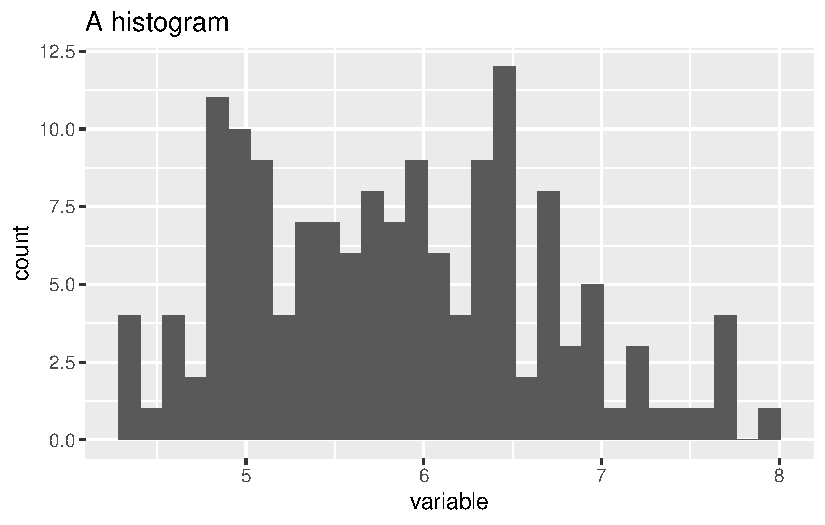
\includegraphics{_data_viz_files/figure-pdf/unnamed-chunk-10-1.pdf}

}

\end{figure}

\hypertarget{start-layering}{%
\subsection{Start layering}\label{start-layering}}

\begin{Shaded}
\begin{Highlighting}[]
\NormalTok{df\_lifetime }\SpecialCharTok{|\textgreater{}} \FunctionTok{ggplot}\NormalTok{(}\FunctionTok{aes}\NormalTok{(ff)) }\CommentTok{\# aes = \textquotesingle{}aesthetic\textquotesingle{}}
\end{Highlighting}
\end{Shaded}

\begin{figure}[H]

{\centering 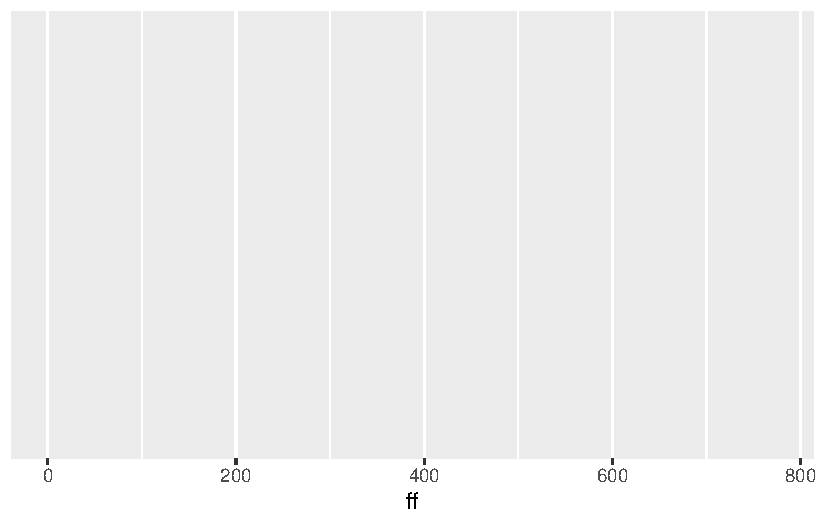
\includegraphics{_data_viz_files/figure-pdf/unnamed-chunk-11-1.pdf}

}

\end{figure}

\hypertarget{add-labels}{%
\subsection{Add labels}\label{add-labels}}

\begin{Shaded}
\begin{Highlighting}[]
\NormalTok{df\_lifetime }\SpecialCharTok{|\textgreater{}} \FunctionTok{ggplot}\NormalTok{(}\FunctionTok{aes}\NormalTok{(ff)) }\SpecialCharTok{+} 
  \FunctionTok{labs}\NormalTok{(}\AttributeTok{title =} \StringTok{"Histogram of first fixataion times"}\NormalTok{,}
       \AttributeTok{x =} \StringTok{"First fixation times (ms)"}\NormalTok{)}
\end{Highlighting}
\end{Shaded}

\begin{figure}[H]

{\centering 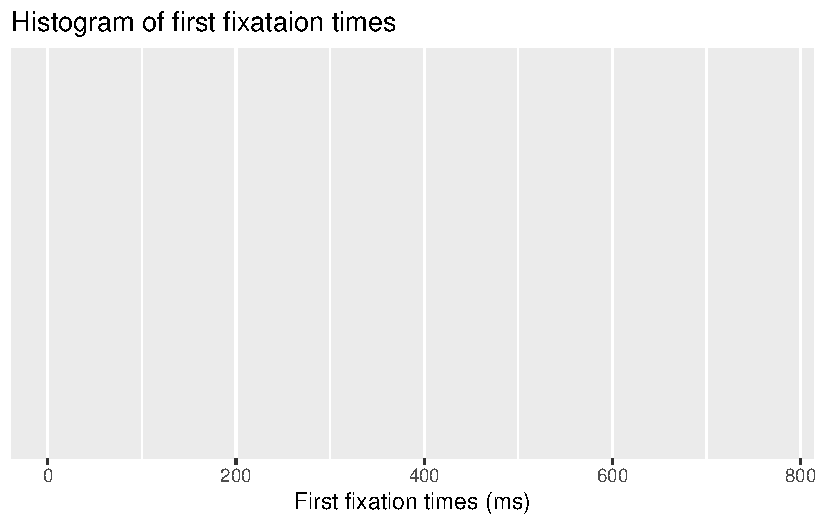
\includegraphics{_data_viz_files/figure-pdf/unnamed-chunk-12-1.pdf}

}

\end{figure}

\hypertarget{add}{%
\subsection{Add}\label{add}}

\begin{Shaded}
\begin{Highlighting}[]
\NormalTok{df\_lifetime }\SpecialCharTok{|\textgreater{}} \FunctionTok{ggplot}\NormalTok{(}\FunctionTok{aes}\NormalTok{(ff)) }\SpecialCharTok{+} 
  \FunctionTok{labs}\NormalTok{(}\AttributeTok{title =} \StringTok{"Histogram of first fixataion times"}\NormalTok{,}
       \AttributeTok{x =} \StringTok{"First fixation times (ms)"}\NormalTok{) }\SpecialCharTok{+}
  \FunctionTok{geom\_histogram}\NormalTok{()}
\end{Highlighting}
\end{Shaded}

\begin{figure}[H]

{\centering 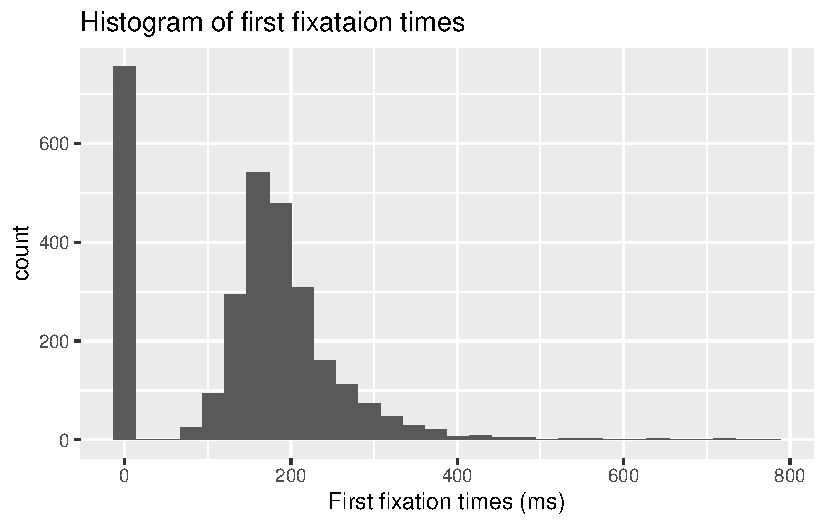
\includegraphics{_data_viz_files/figure-pdf/unnamed-chunk-13-1.pdf}

}

\caption{Distribution of first fixation times at the verb region (raw
milliseconds)}

\end{figure}

\hypertarget{add-condition}{%
\subsection{Add condition}\label{add-condition}}

\begin{Shaded}
\begin{Highlighting}[]
\NormalTok{df\_lifetime }\SpecialCharTok{|\textgreater{}} \FunctionTok{ggplot}\NormalTok{(}\FunctionTok{aes}\NormalTok{(ff, }\AttributeTok{fill =}\NormalTok{ condition)) }\SpecialCharTok{+} 
  \FunctionTok{labs}\NormalTok{(}\AttributeTok{title =} \StringTok{"First fixataion times at the verb region"}\NormalTok{,}
       \AttributeTok{x =} \StringTok{"First fixation times (ms)"}\NormalTok{) }\SpecialCharTok{+}
  \FunctionTok{geom\_histogram}\NormalTok{()}
\end{Highlighting}
\end{Shaded}

\begin{figure}[H]

{\centering 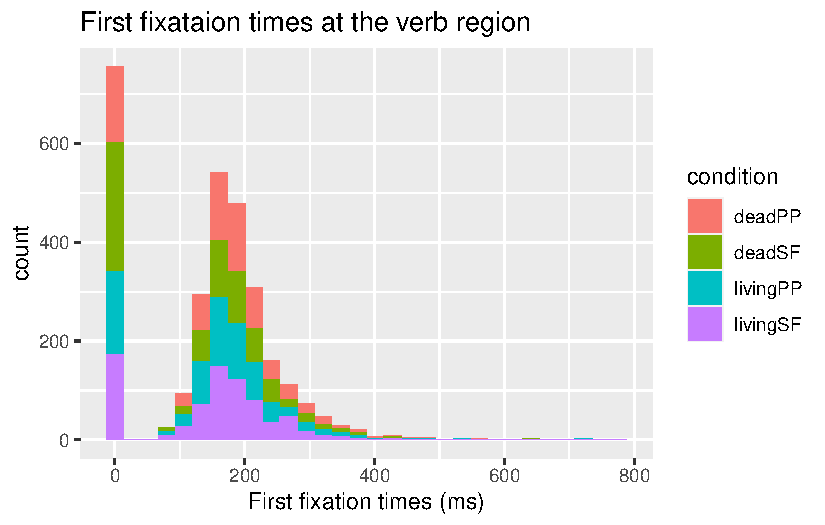
\includegraphics{_data_viz_files/figure-pdf/unnamed-chunk-14-1.pdf}

}

\caption{Distribution of first fixation times at the verb region (raw
milliseconds)}

\end{figure}

The colour here is STACKED!! i.e., not layered. Notice the distribution
doesn't change from all grey to coloured

\hypertarget{customisation}{%
\subsection{Customisation}\label{customisation}}

\begin{itemize}
\tightlist
\item
  we can add arguments to our geoms

  \begin{itemize}
  \tightlist
  \item
    e.g., transparency: \texttt{alpha\ =} takes a value between 0 to 1
  \end{itemize}
\item
  we can use \texttt{theme()} to customise font sizes, legend placement,
  etc.
\item
  tehre are also popular preset themes, such as \texttt{theme\_bw()} and
  \texttt{theme\_minimal()}
\end{itemize}

\subsubsection{\texorpdfstring{\texttt{theme\_bw()}}{theme\_bw()}}

\begin{Shaded}
\begin{Highlighting}[numbers=left,,]
\NormalTok{df\_lifetime }\SpecialCharTok{|\textgreater{}} \FunctionTok{ggplot}\NormalTok{(}\FunctionTok{aes}\NormalTok{(ff, }\AttributeTok{fill =}\NormalTok{ condition)) }\SpecialCharTok{+} 
  \FunctionTok{labs}\NormalTok{(}\AttributeTok{title =} \StringTok{"Histogram of first fixataion times"}\NormalTok{,}
       \AttributeTok{x =} \StringTok{"First fixation times (ms)"}\NormalTok{) }\SpecialCharTok{+}
  \FunctionTok{geom\_histogram}\NormalTok{(}\AttributeTok{alpha=}\NormalTok{.}\DecValTok{5}\NormalTok{) }\SpecialCharTok{+}
  \FunctionTok{theme\_bw}\NormalTok{()}
\end{Highlighting}
\end{Shaded}

\begin{figure}[H]

{\centering 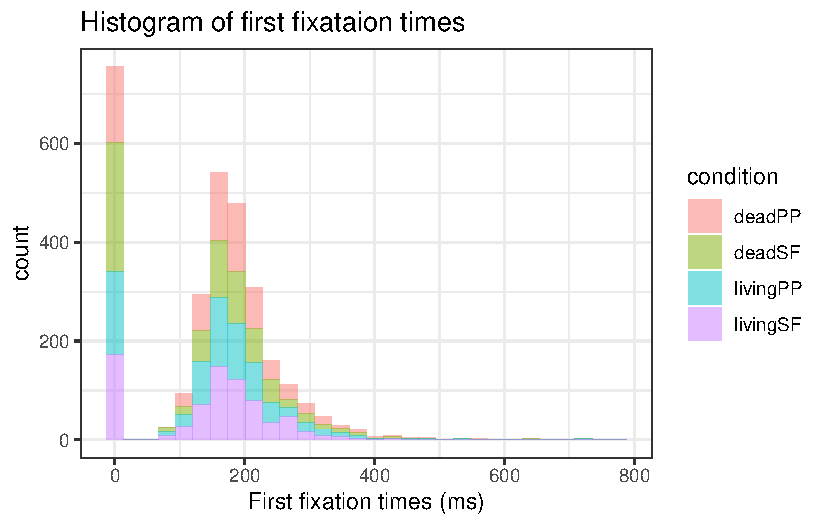
\includegraphics{_data_viz_files/figure-pdf/unnamed-chunk-15-1.pdf}

}

\caption{Distribution of first fixation times at the verb region (raw
milliseconds).}

\end{figure}

\subsubsection{\texorpdfstring{\texttt{theme\_minimal()}}{theme\_minimal()}}

\begin{Shaded}
\begin{Highlighting}[numbers=left,,]
\NormalTok{df\_lifetime }\SpecialCharTok{|\textgreater{}} \FunctionTok{ggplot}\NormalTok{(}\FunctionTok{aes}\NormalTok{(ff, }\AttributeTok{fill =}\NormalTok{ condition)) }\SpecialCharTok{+} 
  \FunctionTok{labs}\NormalTok{(}\AttributeTok{title =} \StringTok{"Histogram of first fixataion times"}\NormalTok{,}
       \AttributeTok{x =} \StringTok{"First fixation times (ms)"}\NormalTok{) }\SpecialCharTok{+}
  \FunctionTok{geom\_histogram}\NormalTok{(}\AttributeTok{alpha=}\NormalTok{.}\DecValTok{5}\NormalTok{) }\SpecialCharTok{+}
  \FunctionTok{theme\_minimal}\NormalTok{()}
\end{Highlighting}
\end{Shaded}

\begin{figure}[H]

{\centering 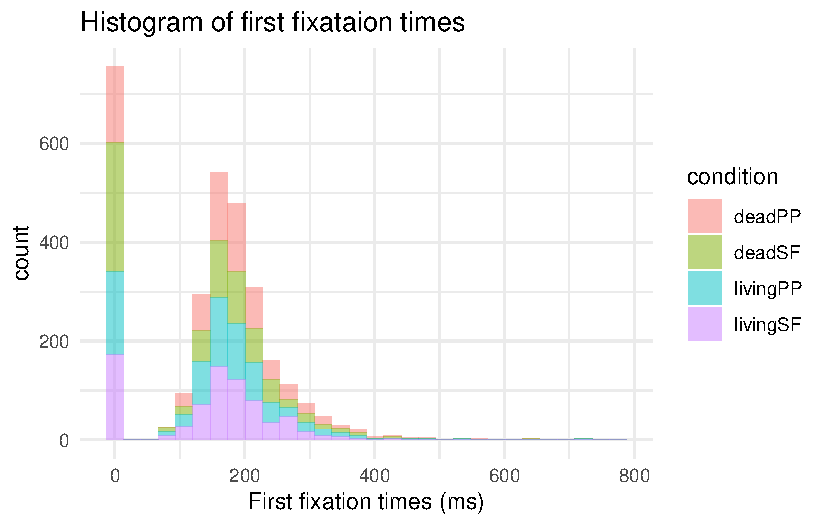
\includegraphics{_data_viz_files/figure-pdf/unnamed-chunk-16-1.pdf}

}

\caption{Distribution of first fixation times at the verb region (raw
milliseconds).}

\end{figure}

\hypertarget{distributions}{%
\section{Distributions}\label{distributions}}

\begin{itemize}
\tightlist
\item
  show the distribution of observations

  \begin{itemize}
  \tightlist
  \item
    so we can see where the data are clustered
  \item
    and eyeball the shape of the distribution
  \end{itemize}
\item
  we already saw the histogram, which shows the number of observations
  per variable value
\item
  \textbf{density plots} are another useful plot for visualising
  distributions
\end{itemize}

\begin{Shaded}
\begin{Highlighting}[]
\NormalTok{iris }\SpecialCharTok{|\textgreater{}} 
  \FunctionTok{ggplot}\NormalTok{(}\FunctionTok{aes}\NormalTok{(}\AttributeTok{x=}\NormalTok{Sepal.Length)) }\SpecialCharTok{+}
  \FunctionTok{geom\_density}\NormalTok{() }\SpecialCharTok{+}
  \FunctionTok{labs}\NormalTok{(}\AttributeTok{title =} \StringTok{"A density plot"}\NormalTok{,}
       \AttributeTok{x =} \StringTok{"variable"}\NormalTok{)}
\end{Highlighting}
\end{Shaded}

\begin{figure}[H]

{\centering 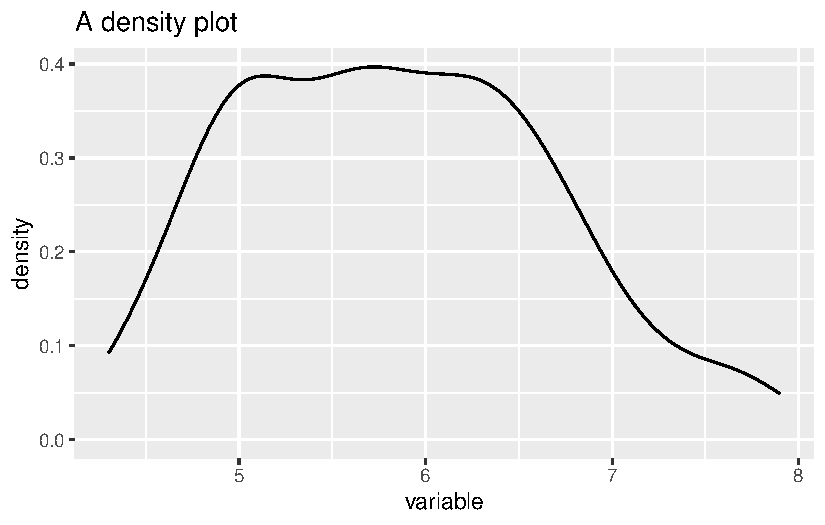
\includegraphics{_data_viz_files/figure-pdf/unnamed-chunk-17-1.pdf}

}

\end{figure}

\hypertarget{density-plots}{%
\subsection{Density plots}\label{density-plots}}

\begin{itemize}
\tightlist
\item
  below I just replaced \texttt{geom\_histogram()} with
  \texttt{geom\_density()}

  \begin{itemize}
  \tightlist
  \item
    I also filtered the data to include only values of \texttt{ff} above
    0
  \end{itemize}
\item
  what is plotted along the y-axis? how does this differ from a
  histogram?
\end{itemize}

\begin{Shaded}
\begin{Highlighting}[numbers=left,,]
\NormalTok{df\_lifetime }\SpecialCharTok{|\textgreater{}} 
  \FunctionTok{filter}\NormalTok{(ff }\SpecialCharTok{\textgreater{}} \DecValTok{0}\NormalTok{) }\SpecialCharTok{|\textgreater{}} 
  \FunctionTok{ggplot}\NormalTok{(}\FunctionTok{aes}\NormalTok{(ff)) }\SpecialCharTok{+} 
  \FunctionTok{labs}\NormalTok{(}\AttributeTok{title =} \StringTok{"Histogram of first fixataion times"}\NormalTok{,}
       \AttributeTok{x =} \StringTok{"First fixation times (ms)"}\NormalTok{) }\SpecialCharTok{+}
  \FunctionTok{geom\_density}\NormalTok{() }\SpecialCharTok{+}
  \FunctionTok{theme\_minimal}\NormalTok{()}
\end{Highlighting}
\end{Shaded}

\begin{figure}[H]

{\centering 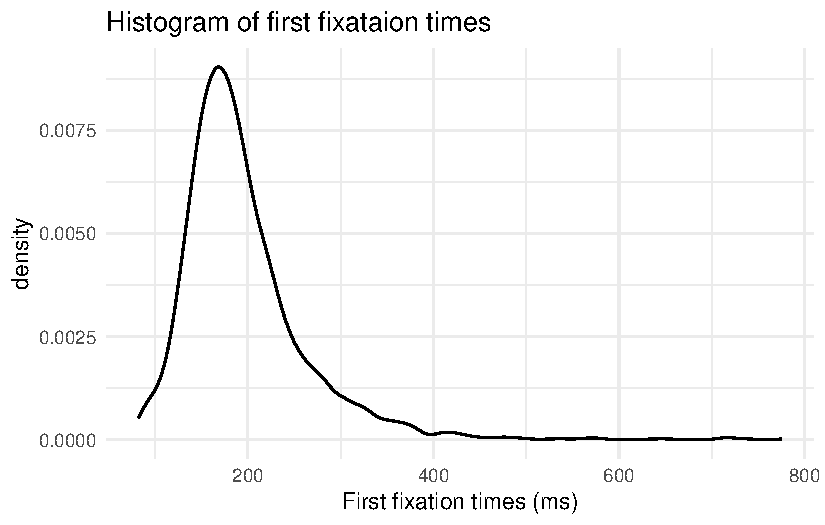
\includegraphics{_data_viz_files/figure-pdf/unnamed-chunk-18-1.pdf}

}

\caption{Distribution of first fixation times at the verb region (raw
milliseconds).}

\end{figure}

\hypertarget{grouped-density-plots}{%
\subsection{Grouped density plots}\label{grouped-density-plots}}

\begin{itemize}
\tightlist
\item
  just like with histograms, we can look at the density plots of
  different subsets of the data with \texttt{aes(fill\ =\ )}

  \begin{itemize}
  \tightlist
  \item
    like region
  \end{itemize}
\end{itemize}

\begin{Shaded}
\begin{Highlighting}[numbers=left,,]
\NormalTok{df\_lifetime }\SpecialCharTok{|\textgreater{}} 
  \FunctionTok{filter}\NormalTok{(ff }\SpecialCharTok{\textgreater{}} \DecValTok{0}\NormalTok{) }\SpecialCharTok{|\textgreater{}} 
  \FunctionTok{ggplot}\NormalTok{(}\FunctionTok{aes}\NormalTok{(ff, }\AttributeTok{fill =}\NormalTok{ region)) }\SpecialCharTok{+} 
  \FunctionTok{labs}\NormalTok{(}\AttributeTok{title =} \StringTok{"Histogram of first fixataion times"}\NormalTok{,}
       \AttributeTok{x =} \StringTok{"First fixation times (ms)"}\NormalTok{) }\SpecialCharTok{+}
  \FunctionTok{geom\_density}\NormalTok{(}\AttributeTok{alpha=}\NormalTok{.}\DecValTok{5}\NormalTok{) }\SpecialCharTok{+}
  \FunctionTok{theme\_minimal}\NormalTok{()}
\end{Highlighting}
\end{Shaded}

\begin{figure}[H]

{\centering 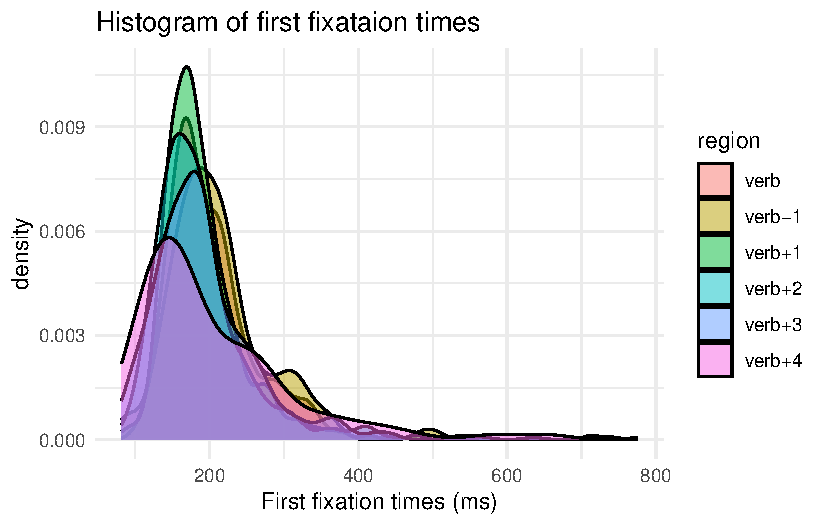
\includegraphics{_data_viz_files/figure-pdf/unnamed-chunk-19-1.pdf}

}

\caption{Distribution of first fixation times at the verb region (raw
milliseconds).}

\end{figure}

\hypertarget{facet_grid}{%
\subsubsection{\texorpdfstring{\texttt{facet\_grid()}}{facet\_grid()}}\label{facet_grid}}

\begin{itemize}
\tightlist
\item
  there are a lot of overlapping density curves, let's try to separate
  them with \texttt{facet\_grid(x\textasciitilde{}y)}
\end{itemize}

\begin{Shaded}
\begin{Highlighting}[numbers=left,,]
\NormalTok{df\_lifetime }\SpecialCharTok{|\textgreater{}} 
  \FunctionTok{filter}\NormalTok{(ff }\SpecialCharTok{\textgreater{}} \DecValTok{0}\NormalTok{) }\SpecialCharTok{|\textgreater{}} 
  \FunctionTok{ggplot}\NormalTok{(}\FunctionTok{aes}\NormalTok{(ff, }\AttributeTok{fill =}\NormalTok{ region)) }\SpecialCharTok{+} 
  \FunctionTok{facet\_grid}\NormalTok{(.}\SpecialCharTok{\textasciitilde{}}\NormalTok{region) }\SpecialCharTok{+}
  \FunctionTok{labs}\NormalTok{(}\AttributeTok{title =} \StringTok{"Density plot of first fixataion times by region"}\NormalTok{,}
       \AttributeTok{x =} \StringTok{"First fixation times (ms)"}\NormalTok{) }\SpecialCharTok{+}
  \FunctionTok{geom\_density}\NormalTok{(}\AttributeTok{alpha=}\NormalTok{.}\DecValTok{5}\NormalTok{) }\SpecialCharTok{+}
  \FunctionTok{theme\_bw}\NormalTok{()}
\end{Highlighting}
\end{Shaded}

\begin{figure}[H]

{\centering 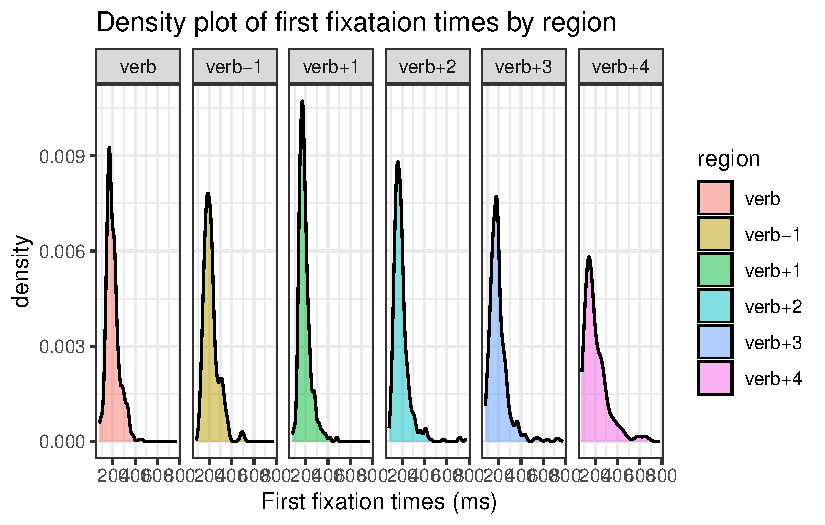
\includegraphics{_data_viz_files/figure-pdf/unnamed-chunk-20-1.pdf}

}

\caption{Distribution of first fixation times at the verb region (raw
milliseconds).}

\end{figure}

\begin{itemize}
\tightlist
\item
  how would you describe the density plots of the different regions?
\end{itemize}

\hypertarget{re-ordering-factors}{%
\subsubsection{re-ordering factors}\label{re-ordering-factors}}

\begin{itemize}
\tightlist
\item
  by default, factors will be ordered alphabetically

  \begin{itemize}
  \tightlist
  \item
    but we don't always want that
  \item
    here, \texttt{verb-1} should be before \texttt{verb}
  \end{itemize}
\end{itemize}

\begin{Shaded}
\begin{Highlighting}[]
\NormalTok{df\_lifetime }\OtherTok{\textless{}{-}}\NormalTok{ df\_lifetime }\SpecialCharTok{\%\textgreater{}\%}
  \FunctionTok{mutate}\NormalTok{(}\AttributeTok{region =} \FunctionTok{factor}\NormalTok{(region, }
                         \AttributeTok{levels =} \FunctionTok{c}\NormalTok{(}\StringTok{"verb{-}1"}\NormalTok{,}\StringTok{"verb"}\NormalTok{,}\StringTok{"verb+1"}\NormalTok{,}\StringTok{"verb+2"}\NormalTok{,}\StringTok{"verb+3"}\NormalTok{,}\StringTok{"verb+4"}\NormalTok{)))}

\FunctionTok{summary}\NormalTok{(df\_lifetime}\SpecialCharTok{$}\NormalTok{region)}
\end{Highlighting}
\end{Shaded}

\begin{verbatim}
verb-1   verb verb+1 verb+2 verb+3 verb+4 
   559    559    559    559    559    182 
\end{verbatim}

\hypertarget{exercise-1}{%
\paragraph{Exercise}\label{exercise-1}}

\begin{enumerate}
\def\labelenumi{\arabic{enumi}.}
\tightlist
\item
  create a density plot with the fill colour set to \texttt{condition},
  but:
\end{enumerate}

\begin{itemize}
\tightlist
\item
  subset the data to only include the verb region
\item
  you can decide if you want to use facets or to have the density curves
  overlayed
\item
  your plot should look something like A or B:
\end{itemize}

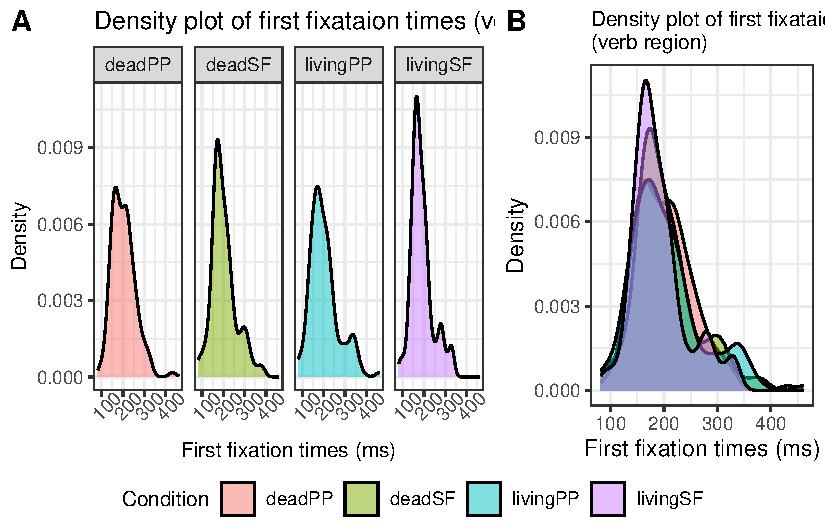
\includegraphics{_data_viz_files/figure-pdf/unnamed-chunk-22-1.pdf}

\hypertarget{extra-exercise}{%
\paragraph{Extra exercise}\label{extra-exercise}}

\begin{enumerate}
\def\labelenumi{\arabic{enumi}.}
\setcounter{enumi}{1}
\tightlist
\item
  Can you produce these plots?
\end{enumerate}

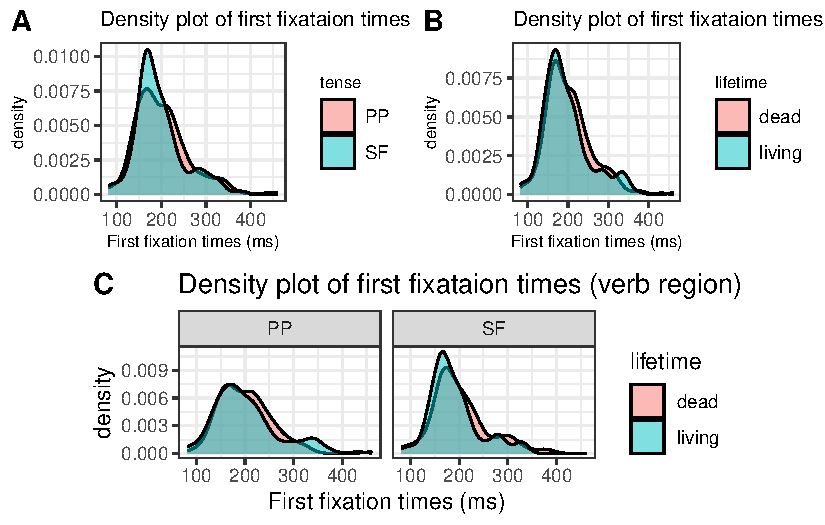
\includegraphics{_data_viz_files/figure-pdf/unnamed-chunk-23-1.pdf}

\hypertarget{scatterplots}{%
\subsection{Scatterplots}\label{scatterplots}}

\begin{itemize}
\tightlist
\item
  histograms and density plots plot a \textbf{single variable} along the
  x-axis

  \begin{itemize}
  \tightlist
  \item
    in most other plots the dependent (measure) variable is plotted
    along the y-axis by convention
  \end{itemize}
\item
  scatterplots plot the relationship between \textbf{two variables}
\end{itemize}

\begin{Shaded}
\begin{Highlighting}[]
\NormalTok{iris }\SpecialCharTok{|\textgreater{}} 
  \FunctionTok{ggplot}\NormalTok{(}\FunctionTok{aes}\NormalTok{(}\AttributeTok{x=}\NormalTok{Sepal.Length, }\AttributeTok{y=}\NormalTok{Sepal.Width)) }\SpecialCharTok{+}
  \FunctionTok{geom\_point}\NormalTok{() }\SpecialCharTok{+}
  \FunctionTok{labs}\NormalTok{(}\AttributeTok{title =} \StringTok{"A scatterplot"}\NormalTok{,}
       \AttributeTok{x =} \StringTok{"variable X"}\NormalTok{,}
       \AttributeTok{y =} \StringTok{"variable Y"}\NormalTok{)}
\end{Highlighting}
\end{Shaded}

\begin{figure}[H]

{\centering 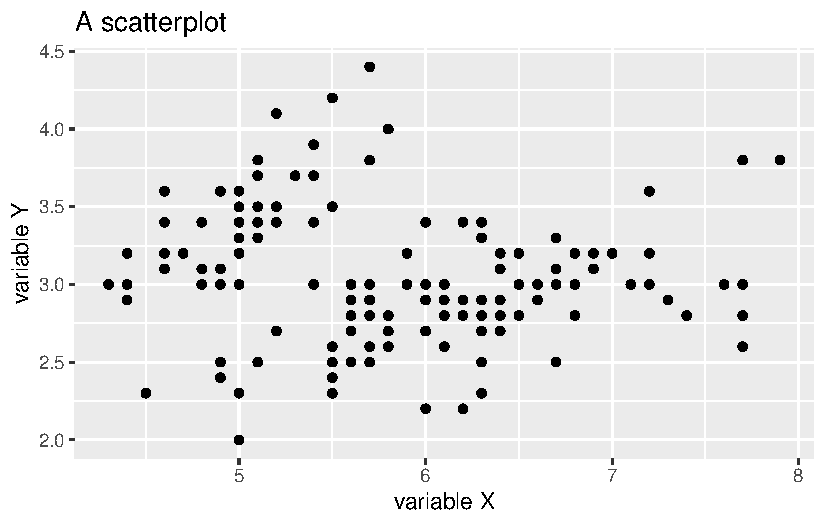
\includegraphics{_data_viz_files/figure-pdf/unnamed-chunk-24-1.pdf}

}

\end{figure}

\hypertarget{scatterplots-1}{%
\subsubsection{Scatterplots}\label{scatterplots-1}}

\begin{itemize}
\tightlist
\item
  the figure below plots total reading times (verb region) to the verb
  region (x-axis) and reaction times to the critical sentence (y-axis)

  \begin{itemize}
  \tightlist
  \item
    what does each point represent?
  \item
    how would you describe the relationship between the two variables?
  \end{itemize}
\end{itemize}

\begin{Shaded}
\begin{Highlighting}[numbers=left,,]
\NormalTok{df\_lifetime }\SpecialCharTok{|\textgreater{}}
  \FunctionTok{filter}\NormalTok{(ff }\SpecialCharTok{\textgreater{}} \DecValTok{0}\NormalTok{,}
\NormalTok{         region }\SpecialCharTok{==} \StringTok{"verb"}\NormalTok{) }\SpecialCharTok{|\textgreater{}}
  \FunctionTok{ggplot}\NormalTok{(}\FunctionTok{aes}\NormalTok{(}\AttributeTok{x =}\NormalTok{ tt, }\AttributeTok{y =}\NormalTok{ rt)) }\SpecialCharTok{+}
  \FunctionTok{labs}\NormalTok{(}\AttributeTok{title =} \StringTok{"Scatter plot of total reading times (verb region)}
\StringTok{and reaction times (critical sentence)"}\NormalTok{,}
       \AttributeTok{x =} \StringTok{"Total reading time (ms)"}\NormalTok{,}
       \AttributeTok{y =} \StringTok{"Reaction time (ms)"}\NormalTok{) }\SpecialCharTok{+}
  \FunctionTok{geom\_point}\NormalTok{(}\AttributeTok{alpha =}\NormalTok{ .}\DecValTok{2}\NormalTok{) }\SpecialCharTok{+}
  \FunctionTok{theme\_bw}\NormalTok{()}
\end{Highlighting}
\end{Shaded}

\begin{figure}[H]

{\centering 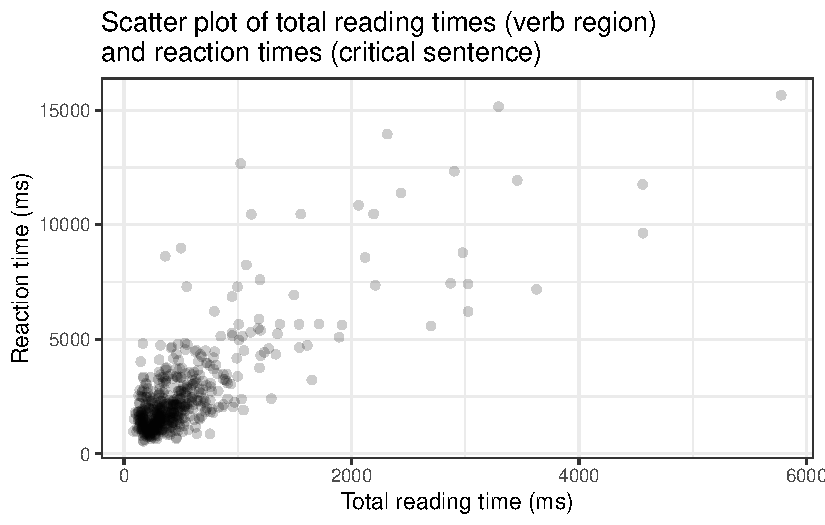
\includegraphics{_data_viz_files/figure-pdf/unnamed-chunk-25-1.pdf}

}

\end{figure}

\hypertarget{exercise-2}{%
\paragraph{Exercise}\label{exercise-2}}

\begin{enumerate}
\def\labelenumi{\arabic{enumi}.}
\tightlist
\item
  Generate a scatterplot of total reading times and reaction times,
  with:

  \begin{itemize}
  \tightlist
  \item
    colour and shape set to condition
  \item
    tip: these both belong in \texttt{aes()}
  \end{itemize}
\item
  What information does this plot suggest?
\end{enumerate}

\hypertarget{summary-statistics}{%
\section{Summary statistics}\label{summary-statistics}}

\begin{itemize}
\tightlist
\item
  measures of location: mean, median, mode
\item
  measures of spread: (interquartile) range, standard deviation
\end{itemize}

\hypertarget{boxplots}{%
\subsection{Boxplots}\label{boxplots}}

\begin{itemize}
\tightlist
\item
  boxplots provide information about the distribution of a
  \emph{continuous} variable

  \begin{itemize}
  \tightlist
  \item
    but includes information like \emph{median} (dark line) and
    \emph{quartiles} (box and whiskers)
  \item
    and \emph{outliers} (dots)
  \end{itemize}
\item
  like scatterplots, require x and y variables

  \begin{itemize}
  \tightlist
  \item
    but one of them needs to be \textbf{categorical}
  \end{itemize}
\end{itemize}

\begin{Shaded}
\begin{Highlighting}[]
\NormalTok{iris }\SpecialCharTok{|\textgreater{}} 
  \FunctionTok{ggplot}\NormalTok{(}\FunctionTok{aes}\NormalTok{(}\AttributeTok{x =}\NormalTok{ Species, }\AttributeTok{y =}\NormalTok{ Sepal.Length)) }\SpecialCharTok{+}
  \FunctionTok{labs}\NormalTok{(}\AttributeTok{title =} \StringTok{"A scatterplot"}\NormalTok{,}
       \AttributeTok{x =} \StringTok{"Categorical variable"}\NormalTok{,}
       \AttributeTok{y =} \StringTok{"Continuous variable"}\NormalTok{) }\SpecialCharTok{+}
  \FunctionTok{geom\_boxplot}\NormalTok{()}
\end{Highlighting}
\end{Shaded}

\begin{figure}[H]

{\centering 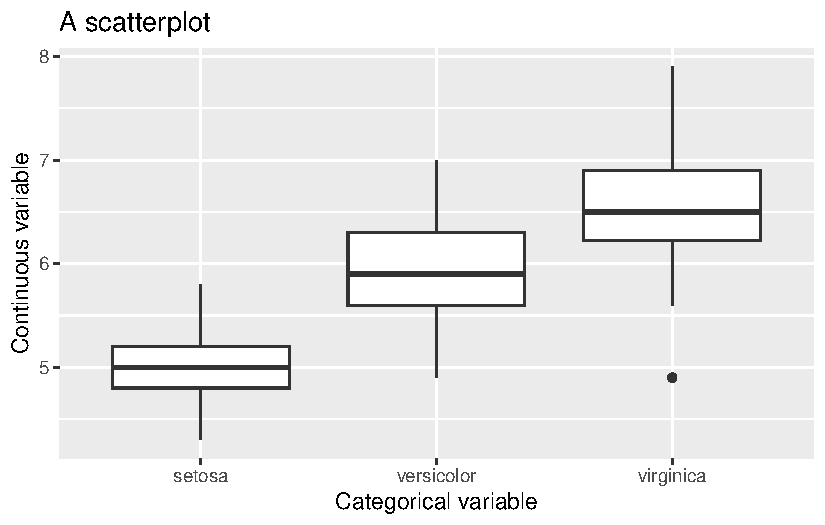
\includegraphics{_data_viz_files/figure-pdf/unnamed-chunk-27-1.pdf}

}

\caption{A scatterplot. Median (50th percentile): thick black lines;
interquartile range (IQR; 25th and 75th percentile): box limits; minimum
(0th percentile) and maximum (100th percentile) excluding outliers: :
whiskers; outliers: points}

\end{figure}

\hypertarget{boxplot-explained}{%
\subsection{Boxplot explained}\label{boxplot-explained}}

\begin{figure}

{\centering 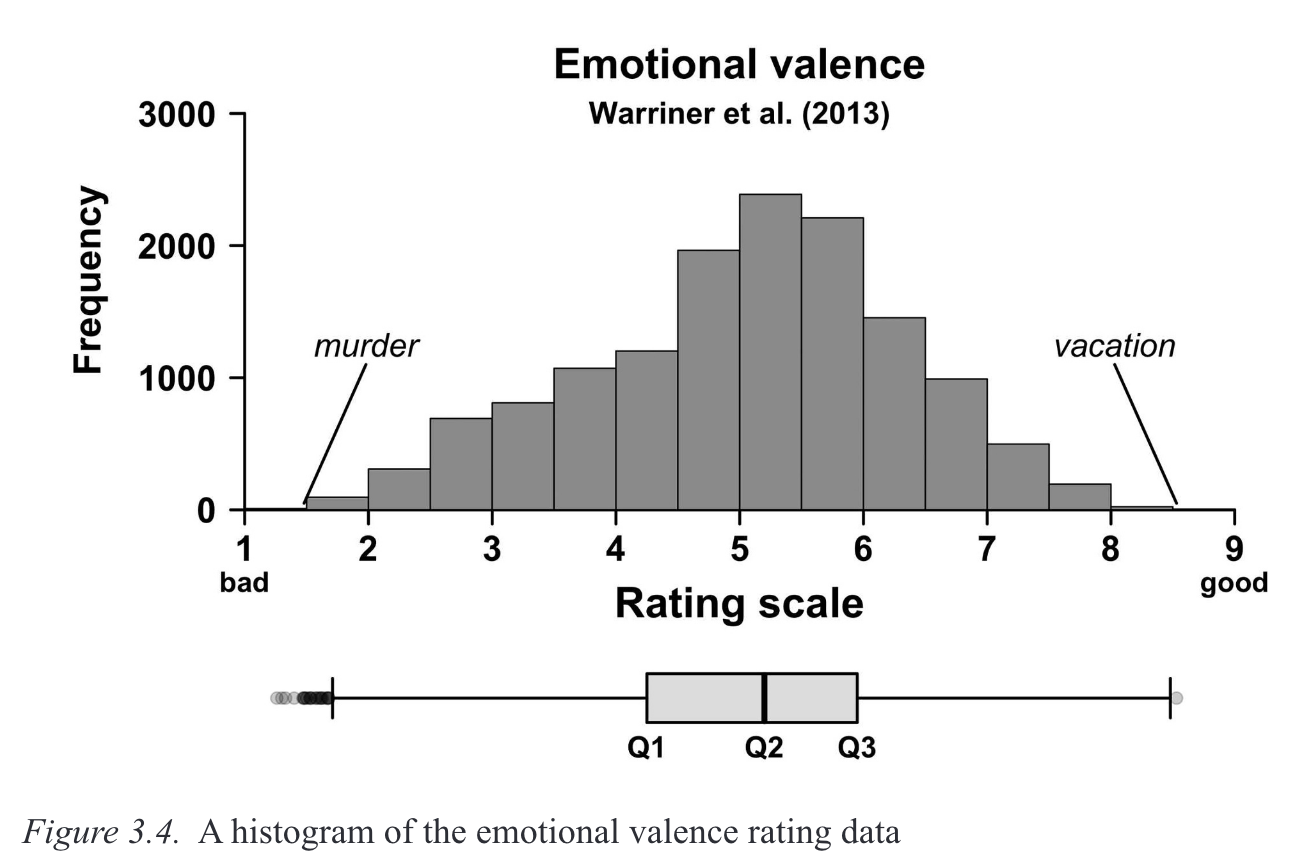
\includegraphics[width=4.32in,height=\textheight]{_data_viz_files/figure-pdf/unnamed-chunk-29-1.png}

}

\caption{Image source: (\textbf{winter\_statistics\_2019?}) (all rights
reserved)}

\end{figure}

\hypertarget{boxplots-1}{%
\subsection{Boxplots}\label{boxplots-1}}

\begin{itemize}
\tightlist
\item
  let's change our scatterplot to a boxplot
\end{itemize}

\begin{Shaded}
\begin{Highlighting}[numbers=left,,]
\NormalTok{df\_lifetime }\SpecialCharTok{|\textgreater{}}
  \FunctionTok{filter}\NormalTok{(ff }\SpecialCharTok{\textgreater{}} \DecValTok{0}\NormalTok{,}
\NormalTok{         region }\SpecialCharTok{==} \StringTok{"verb"}\NormalTok{) }\SpecialCharTok{|\textgreater{}}
  \FunctionTok{ggplot}\NormalTok{(}\FunctionTok{aes}\NormalTok{(}\AttributeTok{x =}\NormalTok{ tense, }\AttributeTok{y =}\NormalTok{ ff)) }\SpecialCharTok{+}
  \FunctionTok{labs}\NormalTok{(}\AttributeTok{title =} \StringTok{"First{-}fixation duration (verb region)"}\NormalTok{,}
       \AttributeTok{x =} \StringTok{"Tense"}\NormalTok{,}
       \AttributeTok{y =} \StringTok{"First{-}fixation duration (ms)"}\NormalTok{) }\SpecialCharTok{+}
  \FunctionTok{geom\_boxplot}\NormalTok{(}\AttributeTok{alpha =}\NormalTok{ .}\DecValTok{2}\NormalTok{) }\SpecialCharTok{+}
  \FunctionTok{theme\_bw}\NormalTok{()}
\end{Highlighting}
\end{Shaded}

\begin{figure}[H]

{\centering 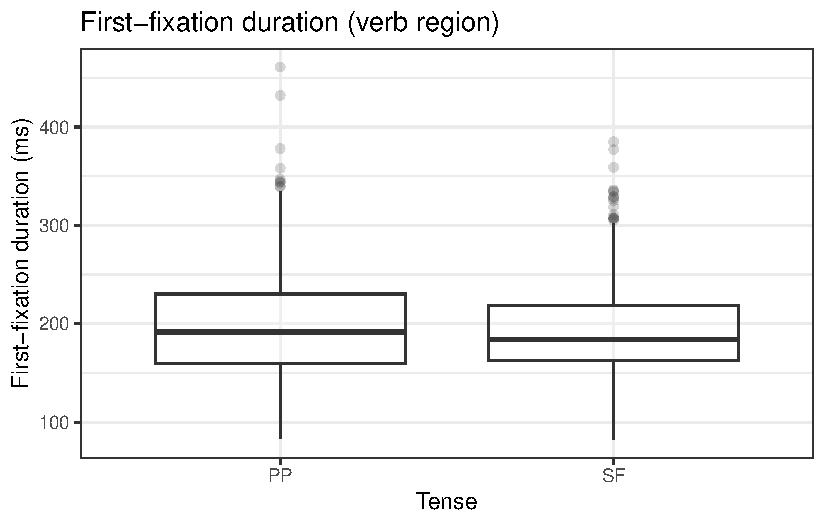
\includegraphics{_data_viz_files/figure-pdf/unnamed-chunk-30-1.pdf}

}

\end{figure}

\hypertarget{grouped-boxplots}{%
\subsubsection{Grouped boxplots}\label{grouped-boxplots}}

\begin{Shaded}
\begin{Highlighting}[numbers=left,,]
\NormalTok{df\_lifetime }\SpecialCharTok{|\textgreater{}}
  \FunctionTok{filter}\NormalTok{(ff }\SpecialCharTok{\textgreater{}} \DecValTok{0}\NormalTok{,}
\NormalTok{         region }\SpecialCharTok{==} \StringTok{"verb"}\NormalTok{) }\SpecialCharTok{|\textgreater{}}
  \FunctionTok{ggplot}\NormalTok{(}\FunctionTok{aes}\NormalTok{(}\AttributeTok{x =}\NormalTok{ tense, }\AttributeTok{y =}\NormalTok{ ff, }\AttributeTok{colour =}\NormalTok{ lifetime)) }\SpecialCharTok{+}
  \FunctionTok{labs}\NormalTok{(}\AttributeTok{title =} \StringTok{"First{-}fixation duration (verb region)"}\NormalTok{,}
       \AttributeTok{x =} \StringTok{"Tense"}\NormalTok{,}
       \AttributeTok{y =} \StringTok{"First{-}fixation duration (ms)"}\NormalTok{) }\SpecialCharTok{+}
  \FunctionTok{geom\_boxplot}\NormalTok{(}\AttributeTok{alpha =}\NormalTok{ .}\DecValTok{2}\NormalTok{) }\SpecialCharTok{+}
  \FunctionTok{theme\_bw}\NormalTok{()}
\end{Highlighting}
\end{Shaded}

\begin{figure}[H]

{\centering 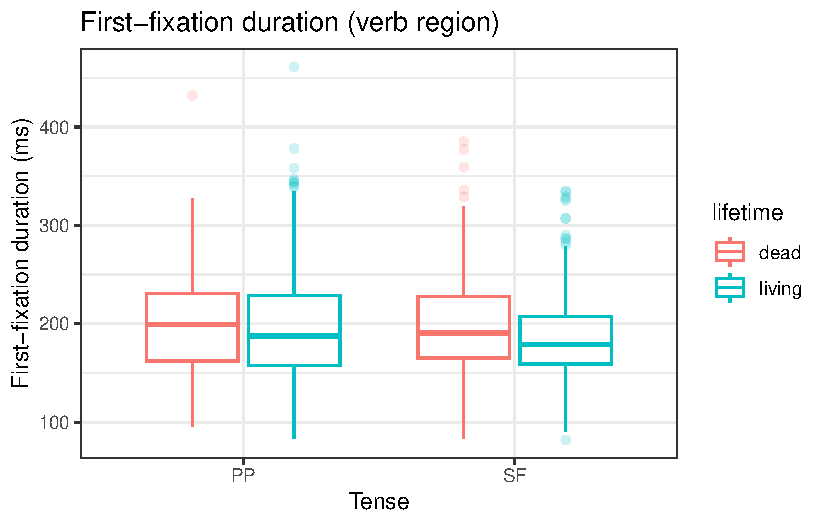
\includegraphics{_data_viz_files/figure-pdf/unnamed-chunk-31-1.pdf}

}

\end{figure}

\hypertarget{exercise-3}{%
\paragraph{Exercise}\label{exercise-3}}

\begin{enumerate}
\def\labelenumi{\arabic{enumi}.}
\tightlist
\item
  Create a group boxplot (x = tense, fill = lifetime) for
\end{enumerate}

\begin{itemize}
\tightlist
\item
  first-pass reading time (verb region)
\item
  regression path duration (verb region)
\item
  total reading time (verb region)
\item
  reaction times (use the \texttt{distinct()} verb to have a single
  observation per participant and per trial)
\end{itemize}

\hypertarget{violin-plots}{%
\subsection{Violin plots}\label{violin-plots}}

\hypertarget{violin-boxplots}{%
\subsection{Violin boxplots}\label{violin-boxplots}}

\hypertarget{summary-statistics-1}{%
\section{Summary statistics}\label{summary-statistics-1}}

\hypertarget{interaction-plots}{%
\subsection{Interaction plots}\label{interaction-plots}}

\begin{itemize}
\tightlist
\item
  common for \textbf{factorial} designs, i.e., comparing
  \emph{categorical} predictors
\item
  there are 2 ways of producing them:

  \begin{itemize}
  \tightlist
  \item
    with your data frame and \texttt{stat\_summary()}
  \item
    or with a summary table and ggplot geoms \texttt{geom\_point()},
    \texttt{geom\_errorbar()}, and \texttt{geom\_line()}
  \end{itemize}
\item
  we'll need our summary table to plot an interaction plot
\end{itemize}

\begin{tabular}{l|l|l|r|r|r|r|r|r|r}
\hline
condition & lifetime & tense & N & mean.ff & sd & se & ci & lower.ci & upper.ci\\
\hline
deadPP & dead & PP & 140 & 198.9 & 57.9 & 4.9 & 9.7 & 189.2 & 208.6\\
\hline
deadSF & dead & SF & 139 & 194.6 & 67.9 & 5.8 & 11.4 & 183.2 & 205.9\\
\hline
livingPP & living & PP & 140 & 194.2 & 77.3 & 6.5 & 12.9 & 181.3 & 207.1\\
\hline
livingSF & living & SF & 140 & 186.0 & 57.6 & 4.9 & 9.6 & 176.4 & 195.6\\
\hline
\end{tabular}

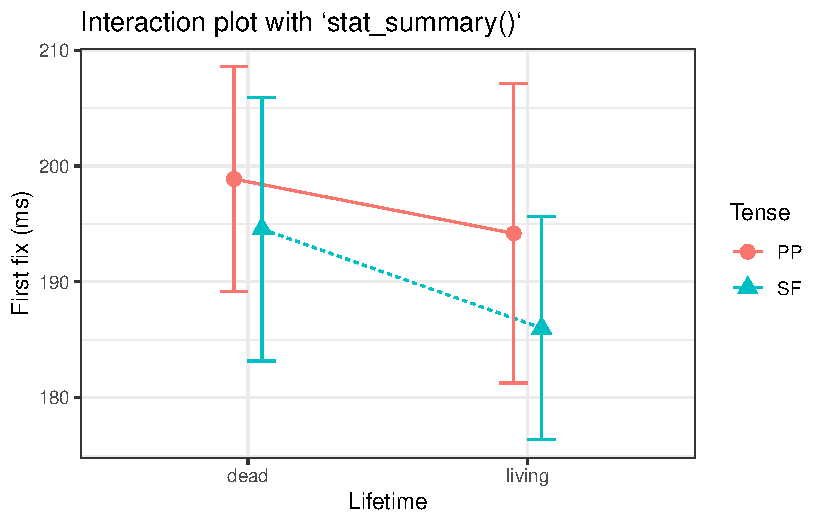
\includegraphics{_data_viz_files/figure-pdf/unnamed-chunk-34-1.pdf}

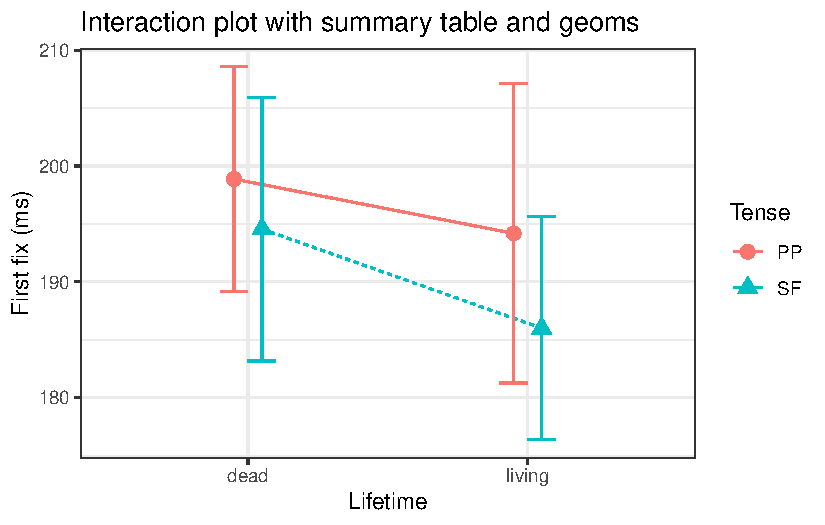
\includegraphics{_data_viz_files/figure-pdf/unnamed-chunk-35-1.pdf}

\hypertarget{binomial-data}{%
\section{Binomial data}\label{binomial-data}}

\begin{itemize}
\tightlist
\item
  binomial data are those with 2 categories, for example

  \begin{itemize}
  \tightlist
  \item
    present, absent
  \item
    yes, no
  \end{itemize}
\item
  in our dataset, each trial ended with a binary naturalness judgement
  task

  \begin{itemize}
  \tightlist
  \item
    how might we plot such data?
  \end{itemize}
\end{itemize}

\hypertarget{bar-plot}{%
\subsection{Bar plot}\label{bar-plot}}

\begin{itemize}
\tightlist
\item
  be sure to read in \texttt{accept} as a factor!
\end{itemize}

\begin{Shaded}
\begin{Highlighting}[]
\NormalTok{df\_lifetime }\SpecialCharTok{|\textgreater{}} 
  \FunctionTok{distinct}\NormalTok{(px,trial,}\AttributeTok{.keep\_all=}\NormalTok{T) }\SpecialCharTok{|\textgreater{}} 
  \FunctionTok{ggplot}\NormalTok{(}\FunctionTok{aes}\NormalTok{(}\AttributeTok{x =} \FunctionTok{as.factor}\NormalTok{(accept) )) }\SpecialCharTok{+}
  \FunctionTok{geom\_bar}\NormalTok{() }\SpecialCharTok{+}
  \FunctionTok{theme\_bw}\NormalTok{()}
\end{Highlighting}
\end{Shaded}

\begin{figure}[H]

{\centering 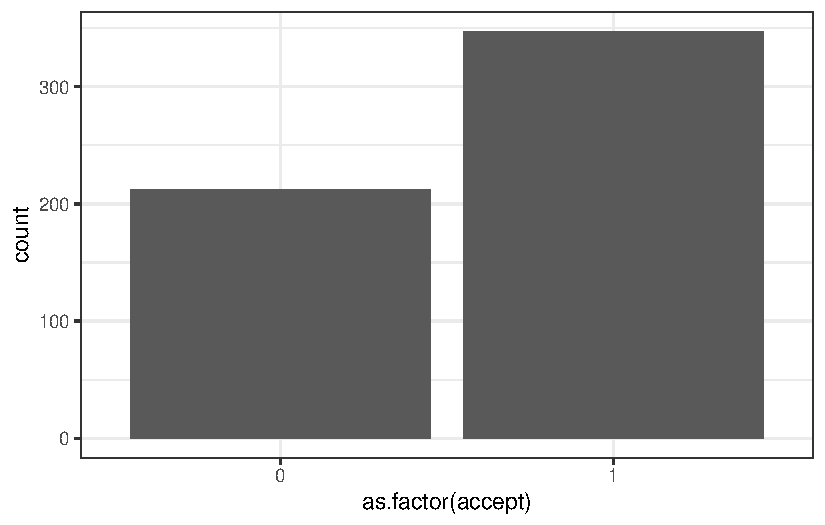
\includegraphics{_data_viz_files/figure-pdf/unnamed-chunk-36-1.pdf}

}

\end{figure}

\begin{Shaded}
\begin{Highlighting}[]
\NormalTok{df\_lifetime }\SpecialCharTok{|\textgreater{}} 
  \FunctionTok{distinct}\NormalTok{(px,trial,}\AttributeTok{.keep\_all=}\NormalTok{T) }\SpecialCharTok{|\textgreater{}} 
  \FunctionTok{ggplot}\NormalTok{(}\FunctionTok{aes}\NormalTok{(}\AttributeTok{x =} \FunctionTok{as.factor}\NormalTok{(accept), }\AttributeTok{fill =}\NormalTok{ condition)) }\SpecialCharTok{+}
  \FunctionTok{labs}\NormalTok{(}\AttributeTok{title =} \StringTok{"Binary responses"}\NormalTok{,}
       \AttributeTok{x =} \StringTok{"Naturalness response"}\NormalTok{,}
       \AttributeTok{fill =} \StringTok{"Condition"}\NormalTok{) }\SpecialCharTok{+}
  \FunctionTok{geom\_bar}\NormalTok{() }\SpecialCharTok{+}
  \FunctionTok{theme\_bw}\NormalTok{()}
\end{Highlighting}
\end{Shaded}

\begin{figure}[H]

{\centering 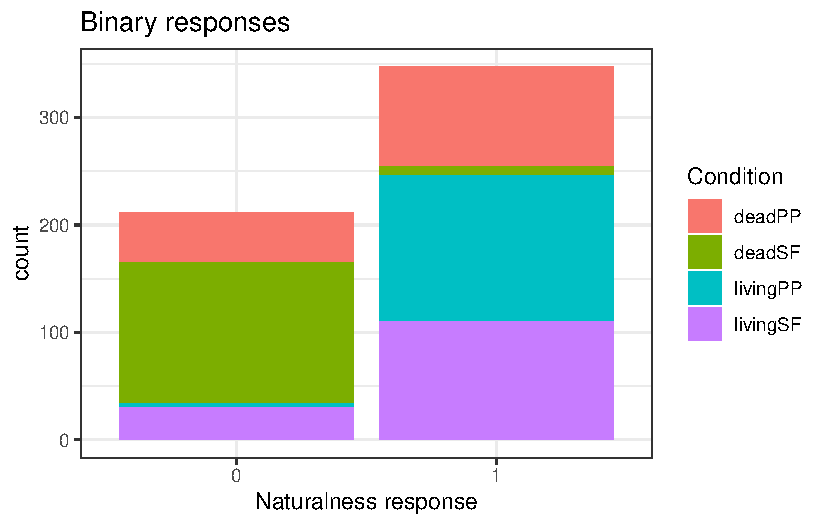
\includegraphics{_data_viz_files/figure-pdf/unnamed-chunk-37-1.pdf}

}

\end{figure}

\hypertarget{grouped-bar-plots}{%
\subsection{Grouped bar plots}\label{grouped-bar-plots}}

\begin{Shaded}
\begin{Highlighting}[]
\NormalTok{df\_lifetime }\SpecialCharTok{|\textgreater{}} 
  \FunctionTok{distinct}\NormalTok{(px,trial,}\AttributeTok{.keep\_all=}\NormalTok{T) }\SpecialCharTok{|\textgreater{}} 
  \FunctionTok{ggplot}\NormalTok{(}\FunctionTok{aes}\NormalTok{(}\AttributeTok{x =} \FunctionTok{as.factor}\NormalTok{(accept), }\AttributeTok{fill =}\NormalTok{ condition)) }\SpecialCharTok{+}
  \FunctionTok{labs}\NormalTok{(}\AttributeTok{title =} \StringTok{"Binary responses"}\NormalTok{,}
       \AttributeTok{x =} \StringTok{"Naturalness response"}\NormalTok{,}
       \AttributeTok{fill =} \StringTok{"Condition"}\NormalTok{) }\SpecialCharTok{+}
  \FunctionTok{geom\_bar}\NormalTok{(}\AttributeTok{position =} \StringTok{"dodge"}\NormalTok{) }\SpecialCharTok{+}
  \FunctionTok{theme\_bw}\NormalTok{()}
\end{Highlighting}
\end{Shaded}

\begin{figure}[H]

{\centering 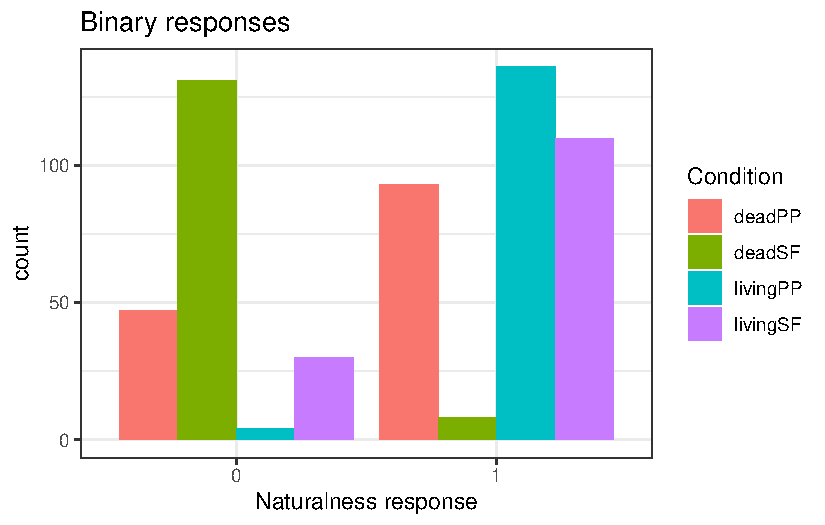
\includegraphics{_data_viz_files/figure-pdf/unnamed-chunk-38-1.pdf}

}

\end{figure}

\hypertarget{exercise-4}{%
\subsubsection{Exercise}\label{exercise-4}}

\begin{enumerate}
\def\labelenumi{\arabic{enumi}.}
\tightlist
\item
  Generate a grouped bar plot (i.e., \texttt{dodge}) with:

  \begin{itemize}
  \tightlist
  \item
    a facet grid for \texttt{tense}
  \item
    plots \texttt{lifetime} on the x-axis
  \item
    and fills the bars based on \texttt{accept}
  \item
    change the labels accordingly
  \item
    customise as you like
  \end{itemize}
\end{enumerate}

\begin{Shaded}
\begin{Highlighting}[]
\NormalTok{df\_lifetime }\SpecialCharTok{|\textgreater{}} 
  \FunctionTok{distinct}\NormalTok{(px,trial,}\AttributeTok{.keep\_all=}\NormalTok{T) }\SpecialCharTok{|\textgreater{}} 
  \FunctionTok{ggplot}\NormalTok{(}\FunctionTok{aes}\NormalTok{(}\AttributeTok{x =}\NormalTok{ lifetime, }\AttributeTok{fill =} \FunctionTok{as.factor}\NormalTok{(accept))) }\SpecialCharTok{+}
  \FunctionTok{facet\_grid}\NormalTok{(.}\SpecialCharTok{\textasciitilde{}}\NormalTok{tense) }\SpecialCharTok{+}
  \FunctionTok{labs}\NormalTok{(}\AttributeTok{title =} \StringTok{"Binary responses"}\NormalTok{,}
       \AttributeTok{x =} \StringTok{"Liftime"}\NormalTok{,}
       \AttributeTok{fill =} \StringTok{"Response"}\NormalTok{) }\SpecialCharTok{+}
  \FunctionTok{geom\_bar}\NormalTok{(}\AttributeTok{position =} \StringTok{"dodge"}\NormalTok{) }\SpecialCharTok{+}
  \FunctionTok{theme\_bw}\NormalTok{()}
\end{Highlighting}
\end{Shaded}

\hypertarget{grouped-bar-plots-1}{%
\subsection{Grouped bar plots}\label{grouped-bar-plots-1}}

\begin{Shaded}
\begin{Highlighting}[]
\NormalTok{df\_lifetime }\SpecialCharTok{|\textgreater{}} 
  \FunctionTok{distinct}\NormalTok{(px,trial,}\AttributeTok{.keep\_all=}\NormalTok{T) }\SpecialCharTok{|\textgreater{}} 
  \FunctionTok{ggplot}\NormalTok{(}\FunctionTok{aes}\NormalTok{(}\AttributeTok{x =}\NormalTok{ lifetime, }\AttributeTok{fill =} \FunctionTok{as.factor}\NormalTok{(accept))) }\SpecialCharTok{+}
  \FunctionTok{facet\_grid}\NormalTok{(.}\SpecialCharTok{\textasciitilde{}}\NormalTok{tense) }\SpecialCharTok{+}
  \FunctionTok{labs}\NormalTok{(}\AttributeTok{title =} \StringTok{"Grouped and faceted barplot"}\NormalTok{,}
       \AttributeTok{x =} \StringTok{"Liftime"}\NormalTok{,}
       \AttributeTok{fill =} \StringTok{"Response"}\NormalTok{) }\SpecialCharTok{+}
  \FunctionTok{geom\_bar}\NormalTok{(}\AttributeTok{position =} \StringTok{"dodge"}\NormalTok{) }\SpecialCharTok{+}
  \FunctionTok{theme\_bw}\NormalTok{()}
\end{Highlighting}
\end{Shaded}

\begin{figure}[H]

{\centering 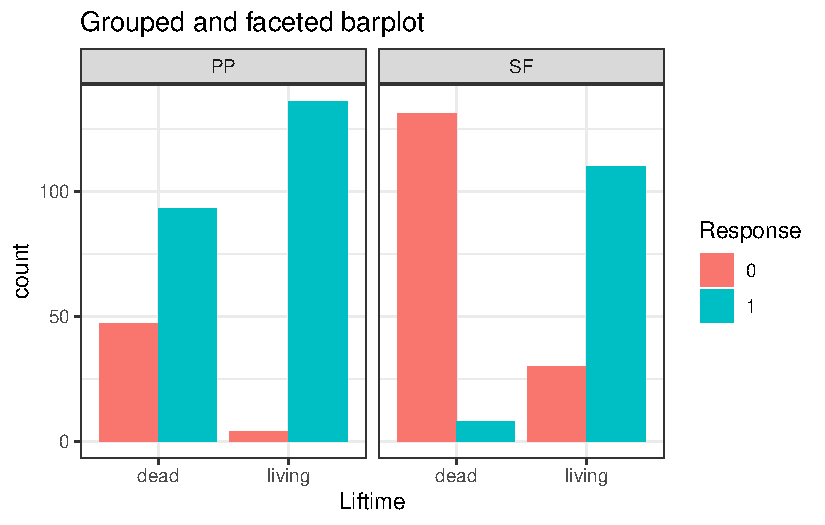
\includegraphics{_data_viz_files/figure-pdf/unnamed-chunk-40-1.pdf}

}

\end{figure}

\hypertarget{stacked-bar-plots}{%
\subsection{Stacked bar plots}\label{stacked-bar-plots}}

\begin{Shaded}
\begin{Highlighting}[numbers=left,,]
\NormalTok{df\_lifetime }\SpecialCharTok{|\textgreater{}} 
  \FunctionTok{distinct}\NormalTok{(px,trial,}\AttributeTok{.keep\_all=}\NormalTok{T) }\SpecialCharTok{|\textgreater{}} 
  \FunctionTok{ggplot}\NormalTok{(}\FunctionTok{aes}\NormalTok{(}\AttributeTok{x =}\NormalTok{ lifetime, }\AttributeTok{fill =} \FunctionTok{as.factor}\NormalTok{(accept))) }\SpecialCharTok{+}
  \FunctionTok{facet\_grid}\NormalTok{(.}\SpecialCharTok{\textasciitilde{}}\NormalTok{tense) }\SpecialCharTok{+}
  \FunctionTok{labs}\NormalTok{(}\AttributeTok{title =} \StringTok{"Stacked and faceted barplot"}\NormalTok{,}
       \AttributeTok{x =} \StringTok{"Liftime"}\NormalTok{,}
       \AttributeTok{fill =} \StringTok{"Response"}\NormalTok{) }\SpecialCharTok{+}
  \FunctionTok{geom\_bar}\NormalTok{(}\AttributeTok{position =} \StringTok{"stack"}\NormalTok{) }\SpecialCharTok{+}
  \FunctionTok{theme\_bw}\NormalTok{()}
\end{Highlighting}
\end{Shaded}

\begin{figure}[H]

{\centering 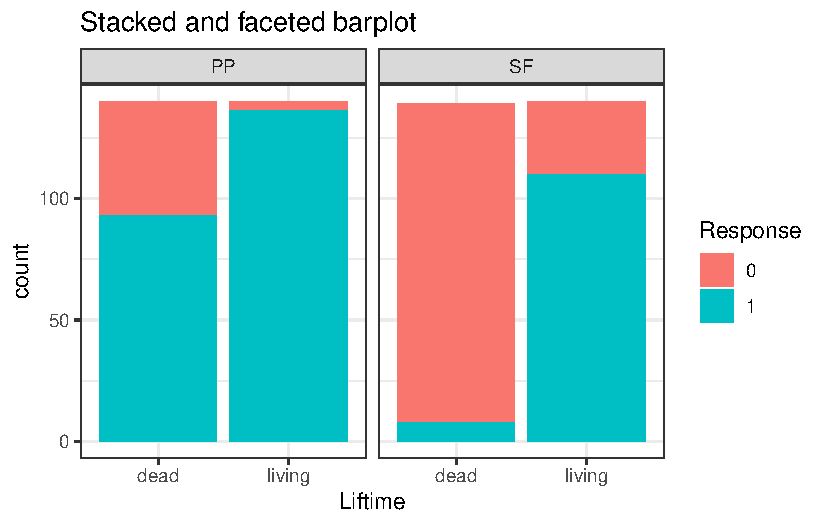
\includegraphics{_data_viz_files/figure-pdf/unnamed-chunk-41-1.pdf}

}

\end{figure}

\hypertarget{exercise-5}{%
\subsubsection{Exercise}\label{exercise-5}}

\begin{enumerate}
\def\labelenumi{\arabic{enumi}.}
\tightlist
\item
  Choose the barplot you like best for binary data
\item
  Reproduce that barplot, but with \texttt{reg\_in} at the
  \texttt{verb1} region
\end{enumerate}

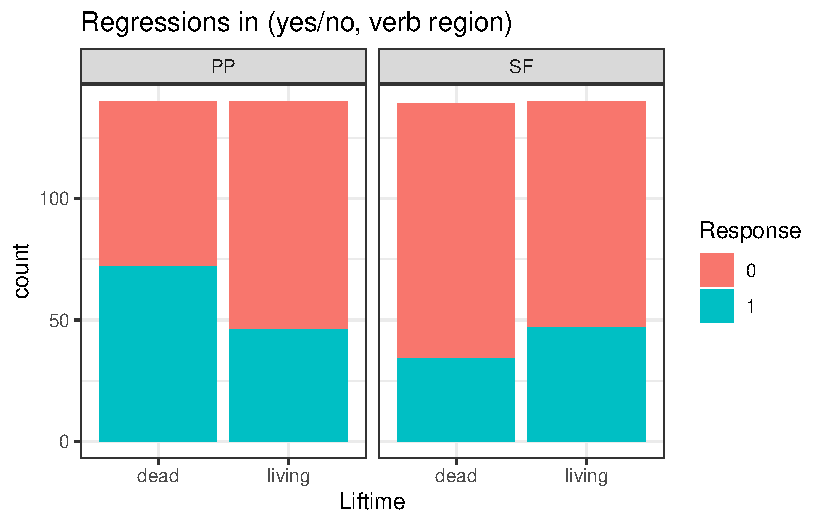
\includegraphics{_data_viz_files/figure-pdf/unnamed-chunk-42-1.pdf}

\hypertarget{extra-exercise-1}{%
\subsubsection{Extra exercise}\label{extra-exercise-1}}

\begin{enumerate}
\def\labelenumi{\arabic{enumi}.}
\tightlist
\item
  Create another bar plot, but for \texttt{reg\_out} for all sentence
  regions
\item
  Use \texttt{facet\_grid()}
\end{enumerate}

\begin{itemize}
\tightlist
\item
  to have facets by region (columns) and by tense (in 2 rows)
\end{itemize}

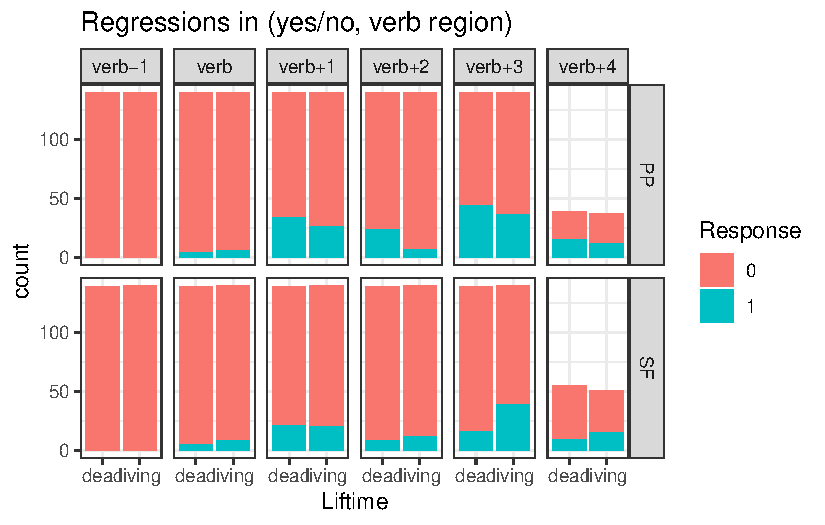
\includegraphics{_data_viz_files/figure-pdf/unnamed-chunk-43-1.pdf}

\hypertarget{resources}{%
\section{Resources}\label{resources}}

Nordmann et al. (2022)

Nordmann \& DeBruine (2022)

Wickham et al. (n.d.),
\href{https://r4ds.hadley.nz/data-visualize.html}{Chapter 2}

\hypertarget{references}{%
\section*{References}\label{references}}

\hypertarget{refs}{}
\begin{CSLReferences}{1}{0}
\leavevmode\vadjust pre{\hypertarget{ref-nordmann_applied_2022}{}}%
Nordmann, E., \& DeBruine, L. (2022). \emph{Applied data skills}
(Version 1.0). Zenodo. \url{https://doi.org/10.5281/zenodo.6365078}

\leavevmode\vadjust pre{\hypertarget{ref-nordmann_data_2022}{}}%
Nordmann, E., McAleer, P., Toivo, W., Paterson, H., \& DeBruine, L. M.
(2022). Data Visualization Using R for Researchers Who Do Not Use R.
\emph{Advances in Methods and Practices in Psychological Science},
\emph{5}(2), 251524592210746.
\url{https://doi.org/10.1177/25152459221074654}

\leavevmode\vadjust pre{\hypertarget{ref-wickham_r_nodate}{}}%
Wickham, H., Çetinkaya-Rundel, M., \& Grolemund, G. (n.d.). \emph{R for
Data Science} (2nd ed.). \url{https://r4ds.hadley.nz/}

\end{CSLReferences}



\end{document}
